% Journal of Science and Law submission
% Andrew H. Bond, San Jose State University
% Built standalone with article class; no special journal template.

\documentclass[11pt]{article}

\usepackage[T1]{fontenc}
\usepackage{lmodern}
\usepackage{amsmath,amssymb,amsfonts,amsthm}
\usepackage[margin=1in]{geometry}
\usepackage{hyperref}
\usepackage{booktabs}
\usepackage{enumitem}
\usepackage{graphicx}
\usepackage{xcolor}
\usepackage{microtype}
\usepackage[round]{natbib}

\hypersetup{colorlinks=true,linkcolor=black,citecolor=blue,urlcolor=blue}

\newtheorem{definition}{Definition}
\newtheorem{proposition}{Proposition}

\title{\bfseries The Legal Bond Index:\\
A Matched-Neighbourhood Diagnostic of Algorithmic\\
Disparity, Applied to COMPAS}

\author{Andrew H.\ Bond\\
Department of Computer Engineering\\
San Jos\'{e} State University, San Jos\'{e}, CA 95192\\
\texttt{andrew.bond@sjsu.edu}\quad ORCID: 0009-0003-2599-6158}

\date{July 2026 (revised)}

\begin{document}
\maketitle

\begin{abstract}
\noindent
The 2016--2017 controversy over the COMPAS pretrial-risk algorithm
exposed a deep ambiguity in the concept of algorithmic fairness.
ProPublica showed that COMPAS's false-positive rate is substantially
higher for Black defendants. Northpointe (the algorithm's vendor)
replied that COMPAS approximately satisfies \emph{predictive parity}:
among defendants it classifies high-risk, the observed recidivism rate
is similar across races. Subsequent technical work
\citep{chouldechova2017,kleinberg2017} proved that the two properties
\emph{cannot both hold} when race-specific recidivism base rates
differ---a genuine impossibility theorem. The literature has since
proliferated competing metrics (demographic parity, equalized odds,
calibration, counterfactual fairness, individual fairness), each
capturing one facet of the problem and none of them dispositive.

We introduce a complementary axis of measurement that the impossibility
result does not constrain: the \emph{Legal Bond Index} (LBI), a
matched-neighbourhood \emph{diagnostic} of algorithmic disparity. For
each defendant, LBI compares the algorithm's score divergence from the
$k$ nearest opposite-group neighbours in a Mahalanobis metric on
selected legitimate predictors (age, prior offences, juvenile record,
charge degree) with its divergence from the $k$ nearest same-group
neighbours; the index is the ratio of the two divergences averaged over
defendants. $\mathrm{LBI} = 1$ means cross-group score divergence among
legitimately-matched neighbours is no larger than within-group
divergence; $\mathrm{LBI} > 1$ means it is larger. For COMPAS
($n = 5{,}278$) the entire neighbourhood-scale curve lies above 1:
$\mathrm{LBI}(\text{race})$ ranges from $1.041$ to $1.069$ across
$k \in [1, 100]$, with pointwise 95\,\% CIs excluding 1 at every
scale; at the illustrative scale $k = 20$,
$\mathrm{LBI}(\text{race}) = 1.049$. We then interrogate that number
the way a sceptical reader should. Cross-race neighbours are indeed
somewhat farther away in feature space than same-race neighbours
(mean distance ratio 1.28 at $k = 20$), and under specifications that
force matching parity---caliper exclusion, coarsened-exact matching,
distance-matched comparators---the point estimate attenuates to
$1.00$--$1.02$. A conditional randomization test that redraws race
labels preserving $P(\text{race} \mid \mathbf{x})$---which a
semi-synthetic validation suite shows is correctly calibrated
(4.5\,\% false-positive rate at the nominal 5\,\% level) exactly where
the conventional permutation test false-fires on 56.5\,\% of race-blind
datasets---still rejects conditional label independence decisively
($z = 4.9$; global multiscale $p = 0.001$). The same validation shows
the index rises monotonically with an injected direct race
coefficient, detects strong proxy discrimination, and can be inflated
by omitting a legitimate predictor from the matching set. The honest
summary is therefore two-sided: COMPAS scores carry a race-associated
component beyond what these legitimate features explain---largest at
ProPublica's medium-or-high classification threshold
($\mathrm{LBI} = 1.092$; matched cross-race vs.\ same-race
disagreement rates 37.3\,\% vs.\ 34.2\,\%)---but the unadjusted index
overstates its magnitude, and we quantify both parts. LBI is a
screening diagnostic conditional on the measured predictors, not a
proof of legal unfairness: because the public dataset contains only
a subset of the variables COMPAS uses, the analysis cannot confirm
that the compared defendants were fully similarly situated, isolate
a causal effect of race, or establish discrimination.

LBI is a matched-neighbourhood disparity diagnostic inspired by
individual-fairness principles and by the Aristotelian
``treat-like-cases-alike'' criterion. It is computationally cheap; it
requires only an audit dataset containing the algorithm's inputs, its
outputs, and the protected attribute (the algorithm itself need not
take the protected attribute as an input); it does not require
knowledge of the algorithm's internals; and it produces a
scale-indexed curve with confidence intervals. It is a
research-stage screening signal that may contribute one input to an
audit, not a validated regulatory audit standard. The reference
implementation is openly archived on
Zenodo (doi:10.5281/zenodo.21310251).
\end{abstract}

\medskip
\noindent\textbf{Keywords:} algorithmic fairness, COMPAS, recidivism
prediction, Mahalanobis distance, matched-pair analysis, criminal
justice, audit, equal protection.

%==============================================================================
\section{Introduction}
\label{sec:intro}
%==============================================================================

In May 2016, ProPublica published an investigation
\citep{angwin2016} arguing that the COMPAS recidivism-risk algorithm,
in use across multiple U.S.\ jurisdictions for pretrial release and
sentencing recommendations, was racially biased against Black
defendants. The reporters' principal evidence was an asymmetry in
error rates: among defendants who did not in fact reoffend within two
years, Black defendants were roughly twice as likely as White
defendants to have been classified as high-risk by COMPAS. Northpointe
(the algorithm's vendor, now equivant) replied that COMPAS was in fact
fair under a different criterion---\emph{predictive parity}: among
defendants it classified high-risk, the empirical recidivism rate was
approximately the same across races \citep{dieterich2016}. Both parties could substantiate their claims
from the same data; the disagreement was about which fairness criterion
applied.

The technical community resolved the empirical question within a year.
\citet{chouldechova2017} and
\citet{kleinberg2017}, working independently,
proved that the two criteria ProPublica and Northpointe each invoked
are \emph{mathematically incompatible} when group-specific base rates
differ: an algorithm that is calibrated within groups
($\Pr(\text{recid} \mid \text{score}, \text{group})$ is invariant
across groups) cannot simultaneously satisfy equalized error rates
(false-positive and false-negative rates invariant across groups),
except in the trivial cases of perfect prediction or equal base
rates. The impossibility is a structural feature of the prediction
problem, not a defect of any particular algorithm.

The decade since has produced a sprawl of competing fairness criteria.
Demographic parity requires that the rate of positive predictions be
equal across groups \citep{feldman2015}. Equalized odds
\citep{hardt2016} requires equal true-positive and false-positive
rates across groups conditional on the actual outcome. Predictive
parity (Northpointe's criterion) requires equal precision across
groups. Counterfactual fairness \citep{kusner2017} requires that an
individual's prediction be invariant under a hypothetical
intervention on their protected attribute. Individual fairness
\citep{dwork2012} requires that similar individuals receive similar
predictions, leaving the similarity metric to be specified. Each
captures a real concern; none of them by itself adjudicates the
COMPAS case; and the proliferation has rendered the debate
\emph{which-metric-to-use} rather than \emph{is-it-fair}.

This paper introduces a diagnostic that is operationally distinct from
all of those above. It is rooted in the oldest legal principle: like
cases should be treated alike. We make this principle precise,
measurable, and applicable to algorithmic systems through the
\emph{Legal Bond Index} (LBI), a matched-neighbourhood diagnostic that
asks whether the algorithm assigns more divergent outputs to defendants
who are similar on the \emph{selected} legitimate predictors but differ
on a protected attribute than to defendants who are similar on both.
LBI is geometric: ``similar'' is operationalized via the Mahalanobis
distance on a feature space of legitimate predictors. LBI is symmetric
across protected attributes and does not depend on the base-rate
structure that drives the calibration--equalized-odds impossibility.

On the ProPublica COMPAS dataset, the primary finding is a
neighbourhood-scale \emph{curve}: at every prespecified scale
$k \in \{1, 5, 10, 20, 50, 100\}$ (where $k$ is the number of nearest
neighbours of each group against which a defendant's score is
compared), $\mathrm{LBI}(\text{race})$ lies above 1, ranging from
$1.041$ to $1.069$ with pointwise 95\,\% CIs excluding 1 at every
scale. At the illustrative scale $k = 20$, used throughout for
detailed diagnostics, $\mathrm{LBI}(\text{race}) = 1.049$: when two
defendants are matched on age, prior offences, juvenile record, and
charge degree, COMPAS scores diverge on average 5\,\% more across
race than within race. A ratio of this kind can be inflated
mechanically---cross-race neighbours might simply be farther away in
feature space than same-race neighbours---and on these data that
concern is partly borne out: we measure the matching gap directly,
show that matching-parity specifications attenuate the point estimate
to $1.00$--$1.02$ (\S\ref{sec:distdiag}), and build the mechanical
component into the null of a conditional randomization test, which
nonetheless rejects race-independence decisively ($z = 4.9$, global
multiscale $p = 0.001$; \S\ref{sec:inferenceresults}). The entire
pipeline---estimator and tests---is validated on semi-synthetic data
with known ground truth (\S\ref{sec:synthetic}).

The remainder of this paper proceeds as follows. Section
\ref{sec:background} reviews the COMPAS controversy and the existing
fairness-metric landscape. Section \ref{sec:lbi} defines LBI formally,
gives the matched-neighbourhood operational specification, and sets
out the inference machinery. Section \ref{sec:empirical} reports the
empirical analysis: filter, features, results, matching diagnostics,
robustness, and the synthetic validation. Section
\ref{sec:discussion} compares LBI to the existing criteria, identifies
what it adds, and discusses limitations. Section \ref{sec:policy}
addresses regulatory and audit implications, including the doctrinal
context. Section \ref{sec:conclusion} concludes.

%==============================================================================
\section{Background: the COMPAS Controversy and the Fairness Landscape}
\label{sec:background}
%==============================================================================

\subsection{The 2016--2017 dispute}

COMPAS (Correctional Offender Management Profiling for Alternative
Sanctions), developed by Northpointe, scores individuals on a 1--10
decile scale of two-year recidivism risk. The algorithm is widely
deployed in U.S.\ pretrial detention decisions. ProPublica's 2016
analysis \citep{angwin2016}, working from public records in Broward
County, Florida, reported two findings: (i) among defendants who did
not reoffend, Black defendants were nearly twice as likely as
White defendants to have been classified as high-risk by COMPAS
(44.9\,\% vs.\ 23.5\,\%); and
(ii) the algorithm's predictive accuracy was approximately equal
across races (about 62\,\% in both groups). The first finding is now
referred to as the \emph{equalized-odds violation}; ProPublica framed
it as evidence of racial bias.

Northpointe's response \citep{dieterich2016} disputed several of
ProPublica's statistical choices, but the company rested its central
defense on a different criterion: it argued that the relevant fairness
criterion was \emph{predictive parity}: among defendants classified
high-risk, the empirical probability of recidivism should be the same
across racial groups. By that criterion COMPAS was approximately fair:
at the high-risk threshold, Black and White defendants had similar
two-year recidivism rates---a precision claim, not a demonstration of
per-score calibration. The dispute, as it played out in the popular and academic
press, was less about the data than about which property a fair
classifier should have.

The technical resolution came rapidly.
\citet{chouldechova2017} proved that an instrument satisfying
predictive parity \emph{cannot} simultaneously satisfy equalized
false-positive and false-negative rates, except in trivial cases.
\citet{kleinberg2017} proved an analogous impossibility theorem for
calibration and balance. The two findings together established that
the COMPAS dispute was not resolvable by data alone: the choice
between Northpointe's criterion and ProPublica's criterion is a
normative choice about which kind of unfairness one prefers to permit.

\subsection{The proliferation of fairness criteria}

The decade since has produced a long list of competing fairness
criteria. We summarize the principal ones to fix terminology.

\textbf{Demographic parity} (\citealp{feldman2015}).
$\Pr(\hat{Y} = 1 \mid A = a) = \Pr(\hat{Y} = 1 \mid A = b)$ for all
protected groups $a, b$. Requires equal positive-prediction rates; this
is generally in tension with using legitimate predictors that correlate
with $A$, though such correlation can sometimes be offset by design
rather than by excluding the predictor. Demographic parity is related
to, but not identical with, the legal doctrine of \emph{disparate
impact}: the doctrine (under Title VII and its progeny) asks whether a
facially neutral practice disproportionately burdens a protected group
\emph{and} whether the practice is justified by business necessity,
a two-step inquiry that no single statistic settles
\citep{barocas2016}. The EEOC's ``four-fifths rule'' is an
administrative enforcement heuristic from employment selection; it has
no doctrinal standing in criminal justice, and we use it in this paper
only as a descriptive yardstick familiar to readers.

\textbf{Equalized odds} (\citealp{hardt2016}).
$\Pr(\hat{Y} = 1 \mid Y = y, A = a) = \Pr(\hat{Y} = 1 \mid Y = y, A
= b)$ for all $y$ and all $a, b$. Requires equal true-positive and
false-positive rates conditional on the true outcome.

\textbf{Predictive parity and calibration} (\citealp{chouldechova2017}).
These are distinct properties. \emph{Calibration} is score-level:
$\Pr(Y = 1 \mid S = s, A = a) = \Pr(Y = 1 \mid S = s, A = b)$ for all
scores $s$ and groups $a, b$ (at a given score the observed outcome rate
is group-independent). \emph{Predictive parity} is a \emph{threshold}
condition on precision: among those \emph{classified} positive,
$\Pr(Y = 1 \mid \hat{Y} = 1, A = a) = \Pr(Y = 1 \mid \hat{Y} = 1, A = b)$.
Northpointe's defence was predictive parity at the high-risk threshold,
not full per-score calibration.

\textbf{Counterfactual fairness} (\citealp{kusner2017}). The
prediction $\hat{Y}(X, A)$ should equal the counterfactual prediction
$\hat{Y}(X_{A := a'}, a')$ for any protected attribute $a'$. Requires
a causal model.

\textbf{Individual fairness} (\citealp{dwork2012}). Similar
individuals should receive similar predictions: a Lipschitz condition
on the prediction map with respect to a task-appropriate metric. The
similarity metric is left to be specified.

The first three criteria are \emph{population-level}: they constrain
aggregate statistics on a population. The fourth requires a causal
model that may not be available. The fifth is general and
philosophically attractive but undertheorized---which metric? The
Legal Bond Index draws on the individual-fairness tradition without
implementing it: it adopts a concrete matching metric (the Mahalanobis
distance on legitimate predictors) and a concrete operational
specification (matched-pair $k$-NN average), turning the
like-cases-alike desideratum into a measurable quantity with a
confidence interval---a diagnostic inspired by the framework, not a
certification of its property (\S\ref{sec:individualfairness}).

\subsection{What population-level metrics miss}

The Chouldechova--Kleinberg impossibility is a result about
\emph{populations}. With unequal base rates, no scoring rule can
simultaneously equalize calibration and false-positive rates across
groups. This is mathematics; one cannot escape it by being clever.

But the impossibility result is silent about \emph{case-level}
properties. Consider the following question: take two defendants who
agree on legitimate predictors (age, priors, juvenile record, charge
degree), differing only on race. Does the algorithm assign them
similar scores? This is a question about \emph{matched pairs}, not
about populations. The Chouldechova--Kleinberg theorem does not
constrain the answer; nothing in the impossibility result prevents
an algorithm from being case-level fair. To the extent the matching features capture the legally relevant grounds
of similarity, an algorithm that scores legitimately-matched defendants
alike is case-level fair, and one that systematically scores them
differently by race exhibits a case-level disparity that the
population-level metrics do not reveal. That qualification is essential:
because the match is on a selected, possibly incomplete set of observed
features, a disparity among matched pairs is a diagnostic signal
requiring further investigation, not by itself proof of legal unfairness
(\S\ref{sec:discussion}, \S\ref{sec:robustness}).

The Legal Bond Index is a quantitative diagnostic aimed at this
matched-comparison question. To be precise about what it delivers: LBI
is computed from local, case-level comparisons and then aggregated, so
the reported index is a population-level summary of matched-neighbourhood
contrasts, not a per-case verdict; and because no defendant's protected
attribute is counterfactually altered---different people are
compared---an elevated LBI establishes that \emph{cross-group score
divergence exceeds within-group score divergence among neighbours
selected on the specified observed features}, not that the algorithm
``uses race.'' It does not adjudicate the Chouldechova--Kleinberg
dispute; it provides a quantitative answer to a question the dispute
does not address.


%==============================================================================
\section{The Legal Bond Index}
\label{sec:lbi}
%==============================================================================

\subsection{Definition}

Let $V$ be the set of individuals (defendants, applicants, claimants)
to whom an algorithm is applied. Each individual $i \in V$ has a
legitimate-predictor vector $\mathbf{x}_i \in \mathbb{R}^d$ and a
protected attribute $g_i \in \{0, 1\}$ (we treat the binary case
throughout and discuss the multi-class extension in
Section~\ref{sec:discussion}). The algorithm assigns a score
$f(i) \in \mathbb{R}$. We equip $\mathbb{R}^d$ with the Mahalanobis
metric
\begin{equation}
\label{eq:mahalanobis}
d_M(\mathbf{x}_i, \mathbf{x}_j) \;=\;
\sqrt{(\mathbf{x}_i - \mathbf{x}_j)^\top \Sigma^{-1} (\mathbf{x}_i - \mathbf{x}_j)},
\end{equation}
where $\Sigma$ is the empirical covariance of $\mathbf{x}$ over the
population. The Mahalanobis metric is the natural choice when
legitimate predictors are correlated (age and prior offences typically
are) because it accounts for the joint distribution rather than
treating each axis independently. Under standardized features,
$d_M$ reduces to Euclidean distance on the de-correlated representation
\citep{mahalanobis1936}.

\begin{definition}[Legal Bond Index, LBI]
\label{def:lbi}
At neighbourhood scale $k \geq 1$, the Legal Bond Index of an
algorithm $f$ with respect to protected attribute $g$ is
\begin{equation}
\label{eq:lbi}
\mathrm{LBI}_k(f, g)
\;=\;
\frac{\mathbb{E}_i \bigl[\, \text{mean}_{j \in N_k(i,\, \neg g_i)} \;
                            \lvert f(i) - f(j) \rvert\, \bigr]}
     {\mathbb{E}_i \bigl[\, \text{mean}_{j \in N_k(i,\, g_i)} \;
                            \lvert f(i) - f(j) \rvert\, \bigr]},
\end{equation}
where $N_k(i, c)$ is the set of the $k$ nearest neighbours to
individual $i$ in $(V, d_M)$ satisfying condition $c$, and
$\mathbb{E}_i$ is the empirical mean over individuals.
\end{definition}

The parameter $k$---the \emph{neighbourhood scale}---is the number of
nearest neighbours of each group against which each defendant's score
is compared: at $k = 1$ each defendant is compared with their single
closest same-group and closest opposite-group neighbour; at $k = 100$
with their hundred closest of each. Small $k$ probes tight matches
(with more sampling noise); large $k$ trades match tightness for
stability. Because no single scale is privileged a priori, we treat
the full curve $k \mapsto \mathrm{LBI}_k$ over prespecified scales as
the primary object of inference, and use $k = 20$ as an illustrative
scale for detailed diagnostics.

\textbf{Interpretation.} The numerator is the average score
difference between an individual and their $k$ nearest neighbours of
the \emph{opposite} protected group. The denominator is the average
score difference between an individual and their $k$ nearest neighbours
of the \emph{same} protected group. The ratio measures cross-group
score divergence relative to within-group score divergence among
neighbours matched on the specified legitimate features:
\begin{itemize}[leftmargin=*]
\item $\mathrm{LBI}_k = 1$: no excess divergence. Scores diverge no
more across the protected attribute than within it, at the same
neighbourhood scale on the same matching features.
\item $\mathrm{LBI}_k > 1$: excess divergence. Defendants' scores
diverge more from legitimately-similar neighbours of the other group
than from equally similar neighbours of their own group. This is a
disparity among comparably-matched cases---a signal to be
investigated. By itself it does not establish that the algorithm uses
the protected attribute: no attribute is counterfactually flipped,
and the excess can also arise from residual differences the matching
features do not capture (\S\ref{sec:distdiag},
\S\ref{sec:synthetic}).
\item $\mathrm{LBI}_k < 1$: deficit divergence. Scores diverge less
across the protected attribute than within it. This is unusual; it
would suggest score variation is compressed across groups relative to
the within-group noise floor.
\end{itemize}

\subsection{Why a ratio, why $k$-NN, and why Mahalanobis}

Each of the three choices in Definition~\ref{def:lbi} is deliberate.

\textbf{Ratio vs.\ raw difference.} The denominator of
\eqref{eq:lbi} provides a within-group baseline against which the
cross-group score gap is normalized. Without this baseline, an
algorithm operating on a population with naturally large legitimate
variation would appear ``unfair'' simply because all neighbourhoods
have large score gaps. The ratio quotients out the algorithm's overall
sensitivity to the \emph{selected} legitimate predictors, contextualizing
the cross-group gap against ordinary within-group variation. It does not
by itself isolate the \emph{marginal causal} contribution of the
protected attribute: that reading holds only to the extent that the
matching features are a sufficiently complete and legally defensible
account of relevant similarity (\S\ref{sec:discussion},
\S\ref{sec:robustness}).

\textbf{$k$-NN matched-pair vs.\ regression.} A regression of $f$ on
legitimate predictors and protected attributes can extract a
coefficient on the protected attribute. But that coefficient depends
on the functional form assumed (linear, polynomial, with
interactions) and on the choice of regularization. The $k$-NN matched-pair
approach is non-parametric: it makes no functional-form assumption
about how $f$ depends on its inputs. It is not, however, assumption-free:
the assumptions are \emph{shifted} to the choice of matching features,
the distance metric, the feature scaling, and $k$, which jointly
determine which cases count as ``similar.'' It also produces a
neighbourhood-scale curve $\mathrm{LBI}_k$ for $k \in [1, 100]$, which
exposes whether the effect is local (small $k$) or global (large $k$).
For COMPAS we find the effect is approximately scale-invariant. This is
suggestive that the pattern is not a small-$k$ artefact, but we read it
cautiously: persistent scale-invariance is equally consistent with a
persistent omitted-variable imbalance as with a genuine case-level
effect.

\textbf{Mahalanobis vs.\ Euclidean.} Legitimate predictors are
correlated (older defendants have more priors, etc.). Euclidean
distance overcounts the contribution of correlated axes; Mahalanobis
de-correlates by construction \citep{mahalanobis1936}. Equivalently,
Mahalanobis distance is Euclidean distance on the whitened
(principal-component, variance-equalized) representation: each
principal direction is divided by its standard deviation, so
high-variance leading directions---which dominate raw Euclidean
distance---are \emph{downweighted} to the common scale, and
disagreement is priced equally per standard deviation along every
de-correlated direction. Section~\ref{sec:robustness} shows the
results are not specific to this choice.

\subsection{Inference: confidence intervals and randomization tests}
\label{sec:inference}

\textbf{Confidence intervals.} LBI is a ratio of means of
per-defendant quantities that are not independent across defendants:
the same individual appears as a neighbour in many other individuals'
comparison sets, so a bootstrap that merely resamples the
per-defendant gaps (holding the neighbourhoods fixed) understates the
resampling variability of the whole construction. We therefore report
percentile-bootstrap confidence intervals in which the neighbourhoods
are \emph{re-formed inside every replicate}: each of 1{,}000
replicates resamples $n$ defendants with replacement, recomputes every
retained defendant's $k$ nearest same-group and opposite-group
neighbours \emph{within the resampled set}, and recomputes the index.
All confidence intervals reported across neighbourhood scales are
\emph{pointwise} (per-$k$), not simultaneous; the multiscale
significance claim rests on the global randomization test below, not
on reading six intervals at once.

\textbf{Randomization tests.} The natural null device is to permute
the protected-attribute labels and recompute LBI; the permutation
distribution supplies an empirical null and the one-sided $p$-value is
the fraction of null draws at or above the observed value. Plain
permutation, however, tests the null that the labels are independent
of \emph{everything}---scores and legitimate features alike. Permuting
race destroys the actual dependence between race and the legitimate
predictors, and it is precisely that dependence which could, in
principle, let a race-blind score produce $\mathrm{LBI} \neq 1$
through differential matching quality. We therefore report three
progressively stricter null constructions, all computed on the full
sample ($n = 5{,}278$) for both the observed and the null statistics,
with 1{,}000 draws each:
\begin{enumerate}[leftmargin=*]
\item \emph{Plain permutation} of the race labels (the conventional
test, reported for continuity);
\item \emph{Stratified permutation} within deciles of the estimated
propensity score $\hat{P}(\text{race} \mid \mathbf{x})$, which
preserves the coarse race--feature dependence; and
\item A \emph{conditional randomization test} (CRT): race labels are
redrawn independently from $\hat{P}(\text{race} \mid \mathbf{x}_i)$
estimated by logistic regression, preserving the race--feature
dependence that permutation destroys. Under this null, any
mechanical contribution of race-correlated feature geometry to the
index is present in the null draws as well.
\end{enumerate}
For the multiscale claim we use a global max-$z$ statistic: each
scale's LBI is standardized against its own null mean and standard
deviation, and the test statistic is the maximum standardized value
over the prespecified scales $k \in \{1, 5, 10, 20, 50, 100\}$; the
global $p$-value compares the observed maximum with the null
distribution of the same maximum. This controls for selection across
scales rather than attaching the significance claim to any single
$k$.

Randomization tests probe the label-independence null; they cannot by
themselves rule out that cross-race neighbours are systematically
worse-matched than same-race neighbours under the \emph{actual}
labels. The direct response to that concern is empirical, and we
treat it as a first-class part of the method: \S\ref{sec:distdiag}
measures the matching-quality gap explicitly and re-estimates LBI
under distance-matched, caliper-restricted, and exact-matched
specifications, and \S\ref{sec:synthetic} calibrates the entire
pipeline---estimator plus tests---on semi-synthetic data with known
ground truth, including race-blind scores on the real,
race-correlated feature distributions.


%==============================================================================
\section{Empirical Analysis: LBI on COMPAS}
\label{sec:empirical}
%==============================================================================

We compute LBI on the ProPublica COMPAS dataset and compare it
against the standard fairness metrics that shaped the 2016--2017
debate.

\subsection{Data and filter}

We use ProPublica's published file
\verb|compas-scores-two-years.csv|, retrieved on June 11 2026 from
the public GitHub repository \verb|propublica/compas-analysis|. The
dataset contains 7,214 records of defendants screened by COMPAS in
Broward County, Florida.

We apply ProPublica's canonical analytical filter to obtain the
6,172-record analysis subset: screening date within 30 days of arrest,
recidivism record present, charge degree not ``Ordinary,'' and COMPAS
score text valid. Restricting further to African-American and
Caucasian defendants (the two race categories that drove the public
controversy and the subsequent technical literature) yields $n =
5{,}278$ defendants, of whom 3,175 (60.2\,\%) are African-American
and 2,103 (39.8\,\%) are Caucasian.

Two definitions used throughout. \emph{Score}: the COMPAS
\emph{general recidivism} decile (\verb|decile_score|, 1--10), not
the separate violent-recidivism scale. COMPAS deciles map to three
published risk categories: 1--4 ``low,'' 5--7 ``medium,'' 8--10
``high.'' \emph{Recidivism}: ProPublica's two-year indicator
(\verb|two_year_recid|)---a new criminal offence resulting in a jail
booking within two years of the COMPAS screening date, excluding
traffic offences and municipal-ordinance violations; it is an
arrest-based outcome, not a conviction-based one, a limitation of
the source data that applies to every study built on this file. The
six matching features contain no missing values in the filtered
subset.

\subsection{Legitimate-feature space}

We adopt six legitimate predictors documented by Northpointe and
engaged by courts as inputs to pretrial risk assessment (see
\emph{State v.\ Loomis}, 881 N.W.2d 749 (Wis.\ 2016), which upheld
sentencing use of COMPAS---whose inputs include criminal-history and
age factors---while cautioning on its use):
\textsf{age}, \textsf{priors\_count}, \textsf{juv\_fel\_count},
\textsf{juv\_misd\_count}, \textsf{juv\_other\_count}, and an
indicator for whether the current charge is a felony
($\mathsf{c\_charge\_F}$). We standardize each feature
(mean-zero, unit-variance) before computing the Mahalanobis metric.
Although these predictors all count prior conduct, they do not
double-count it: the three juvenile counts are mutually exclusive charge
classes (felony, misdemeanour, other), and \textsf{priors\_count} records
adult priors, so the four \emph{partition} rather than duplicate a
defendant's record. The empirical covariance matrix accordingly has
condition number $2.65$, confirming no severe multicollinearity; the
Mahalanobis metric additionally de-correlates whatever residual
dependence remains. The COMPAS score is the published decile risk
($1$--$10$).

\subsection{Standard fairness metrics: confirming the prior literature}

We first reproduce the 2016--2017 controversy by computing standard
metrics on the filtered subset. Table~\ref{tab:standard} reports
the headline numbers.

\begin{table}[h]
\centering
\caption{Standard fairness metrics on the COMPAS Black/White subset
($n{=}5{,}278$). Binary threshold: decile $\geq 5$, ProPublica's
``medium-or-high'' class (see \S\ref{sec:scorerep}); ``high-risk''
in the row labels follows ProPublica's usage.}
\label{tab:standard}
\begin{tabular}{lrrr}
\toprule
\textbf{Metric} & \textbf{African-American} & \textbf{Caucasian} & \textbf{Disparity} \\
\midrule
$n$                   & 3{,}175 & 2{,}103 & --- \\
Base recidivism rate  & 0.523 & 0.391 & $+0.132$ \\
$\Pr(\text{high-risk})$ & 0.576 & 0.331 & $\times\,1.74$ \\
False positive rate   & 0.423 & 0.220 & $+0.203$ \\
False negative rate   & 0.285 & 0.496 & $-0.211$ \\
$\Pr(\text{recid}\mid\text{high-risk})$ & 0.650 & 0.595 & $+0.055$ \\
$\Pr(\text{recid}\mid\text{low-risk})$  & 0.351 & 0.290 & $+0.061$ \\
\bottomrule
\end{tabular}
\end{table}

The pattern matches the published literature exactly. ProPublica's
headline finding---the false-positive-rate disparity---is
$+20.3$ percentage points, with a corresponding false-negative-rate
disparity of $-21.1$ percentage points. (These are distinct rates on
different denominators---the FPR is the complement of the true-negative
rate and the FNR of the true-positive rate---so they are not two forms
of a single quantity, though under this classifier they move in opposite
directions.) Northpointe's defence is \emph{predictive parity} at the
high-risk threshold: the empirical recidivism rate among defendants
classified high-risk is approximately equal across races (a precision
gap of $+0.055$), not a demonstration of per-decile calibration. The
Chouldechova--Kleinberg impossibility holds because the recidivism base
rates differ by $+13.2$ percentage points. (An earlier version of
this table mixed values from differently filtered drafting runs; all
cells are now produced by the same script and subset as every other
number in the paper.)

\subsection{LBI across neighbourhood scales}
\label{sec:lbiresults}

We compute LBI(race) and LBI(sex) at the six prespecified
neighbourhood scales $k \in \{1, 5, 10, 20, 50, 100\}$ using the
matched-neighbourhood $k$-NN procedure of Definition~\ref{def:lbi}.
Confidence intervals come from the bootstrap of
\S\ref{sec:inference}, which re-forms every neighbourhood inside each
of 1{,}000 replicates; they are noticeably wider than the naive
per-defendant bootstrap (at $k = 20$: $[1.027, 1.072]$ vs.\
$[1.039, 1.058]$), which is what one expects once the reuse of
neighbours across defendants (mean 40 reuses, max 198) is allowed to
propagate into the interval. All CIs are pointwise per scale.

\begin{table}[h]
\centering
\caption{Legal Bond Index for COMPAS, by protected attribute and
neighbourhood scale $k$. $n = 5{,}278$ defendants. CIs are
pointwise percentile bootstrap with neighbourhoods re-formed in every
replicate.}
\label{tab:lbi}
\begin{tabular}{rrrrrr}
\toprule
\multicolumn{1}{c}{\textbf{$k$}}
 & \multicolumn{2}{c}{\textbf{LBI(race)}}
 & \multicolumn{2}{c}{\textbf{LBI(sex)}} \\
\cmidrule(lr){2-3}\cmidrule(lr){4-5}
 & value & 95\,\% CI & value & 95\,\% CI \\
\midrule
  1 & 1.045 & $[1.002, 1.089]$ & 0.962 & $[0.935, 1.032]$ \\
  5 & 1.043 & $[1.010, 1.074]$ & 1.012 & $[0.974, 1.043]$ \\
 10 & 1.041 & $[1.017, 1.068]$ & 1.016 & $[0.987, 1.043]$ \\
 20 & 1.049 & $[1.027, 1.072]$ & 1.021 & $[0.998, 1.044]$ \\
 50 & 1.060 & $[1.041, 1.079]$ & 1.028 & $[1.008, 1.048]$ \\
100 & 1.069 & $[1.053, 1.087]$ & 1.041 & $[1.023, 1.060]$ \\
\bottomrule
\end{tabular}
\end{table}

Figure~\ref{fig:lbi-by-attribute} plots the curves. LBI(race) lies
above $1$ at every scale, with pointwise CIs excluding $1$ throughout
(narrowly at $k = 1$, where estimates are dominated by distance ties;
see \S\ref{sec:implementation}). The race curve, not any single
point on it, is the primary finding; $k = 20$ is used below as an
illustrative scale for the detailed diagnostics.

\textbf{The sex result.} LBI(sex) is \emph{not} distinguishable from
$1$ at small and moderate scales: the point estimate is below $1$ at
$k = 1$ ($0.962$) and the pointwise CIs include $1$ for all
$k \leq 20$. Only at $k = 50$ and $100$---scales at which matches are
loose---do the intervals exclude $1$, and the global multiscale
randomization tests of \S\ref{sec:inferenceresults} do not reject
label independence for sex (plain permutation $p = 0.39$, conditional
test $p = 0.90$). An earlier version of this paper described the sex
effect as real but smaller than the race effect; the corrected
inference does not support that claim, and we withdraw it. We note
also that a nonzero LBI(sex) would not carry the same normative
significance as LBI(race): courts have upheld express consideration
of sex in risk assessment (\S\ref{sec:doctrine}), so LBI(sex) is
reported as a methodological comparison, not an alleged violation.

\textbf{Focal-group decomposition.} Averaging over all defendants
weights the larger group (African-American, 60.2\,\%) more heavily.
Computing the index separately by focal group at $k = 20$ gives
$\mathrm{LBI}_{\text{Black focal}} = 1.027$ $[1.015, 1.039]$ and
$\mathrm{LBI}_{\text{White focal}} = 1.087$ $[1.071, 1.102]$; the
group-balanced index (equal-weight average of the two focal groups'
numerators and denominators) is $1.055$. The disparity is thus
asymmetric: White defendants' scores diverge from their matched
Black neighbours substantially more than the reverse, consistent
with matched Black neighbours receiving systematically different
(higher) scores in the neighbourhoods of White focal defendants.

\begin{figure}[h]
\centering
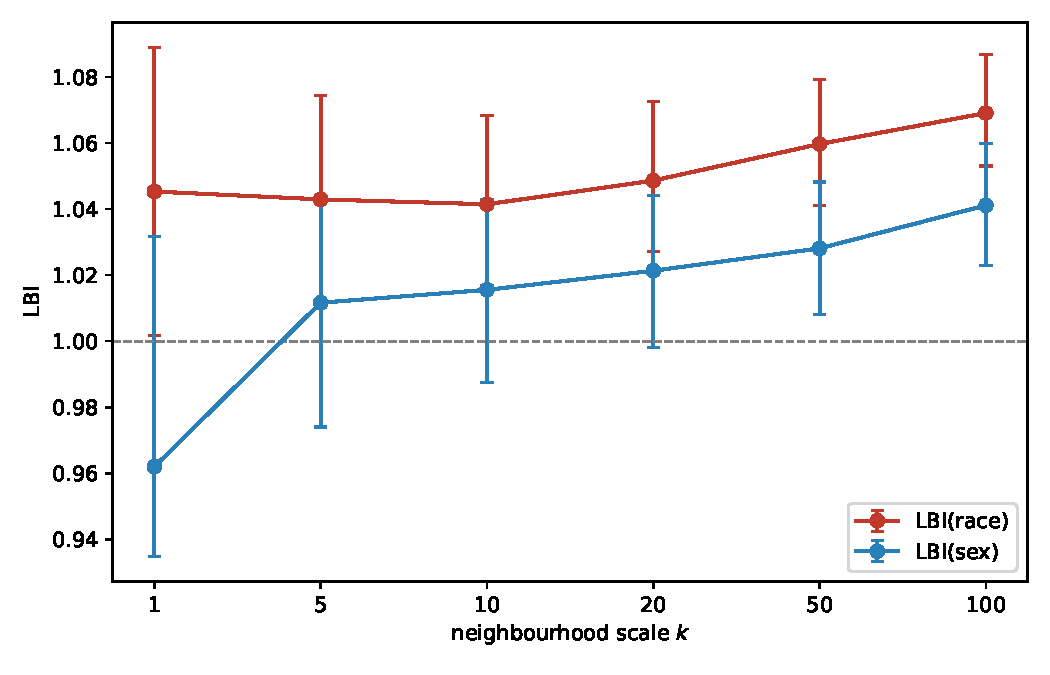
\includegraphics[width=0.75\textwidth]{figures/lbi_by_attribute.pdf}
\caption{COMPAS Legal Bond Index by protected attribute, across
neighbourhood scales $k$. Bars show pointwise 95\,\% bootstrap CIs
with neighbourhoods re-formed in every replicate. The race curve is
above $1$ at every scale; the sex curve is not distinguishable from
$1$ at $k \leq 20$ and its global randomization test does not reject
(\S\ref{sec:inferenceresults}). The horizontal dashed line marks
LBI $= 1$.}
\label{fig:lbi-by-attribute}
\end{figure}

\subsection{Are cross-race neighbours worse-matched?}
\label{sec:distdiag}

Definition~\ref{def:lbi} compares each defendant with two different
neighbour sets, and nothing in the definition forces those sets to be
equally close. If opposite-race neighbours are systematically farther
away in the legitimate-feature space, their scores may differ more
even under a completely race-blind scoring function, mechanically
producing $\mathrm{LBI} > 1$. This subsection measures that gap
directly and re-estimates the index under specifications that force
matching parity. The answer, in brief: the gap is real, it accounts
for part---but not all---of the unadjusted index, and quantifying it
changes the honest summary of the COMPAS result.

\textbf{The matching gap.} Cross-race neighbours are indeed farther
(Table~\ref{tab:distdiag}; Figure~\ref{fig:distdiag}): at $k = 20$
the mean Mahalanobis distance to cross-race neighbours is $0.458$
versus $0.357$ to same-race neighbours, a ratio of $1.28$, shrinking
monotonically with $k$ (from $1.52$ at $k = 1$ to $1.17$ at
$k = 100$); the medians tell the same story ($0.143$ cross vs.\
$0.120$ same at $k = 20$), so the gap is not an artifact of a few
extreme defendants. Per-feature balance shows the same picture: the mean
absolute standardized difference between a defendant and their
cross-race neighbours exceeds the same-race value on every feature,
most markedly on prior counts ($0.187$ vs.\ $0.141$) and juvenile
felony counts ($0.082$ vs.\ $0.046$). Common support, by contrast,
is not a problem: on a logistic propensity score
$\hat{P}(\text{race} \mid \mathbf{x})$, 99.8\,\% of defendants lie in
the common-support interval, and restricting to that region leaves
the index unchanged ($1.048$).

\begin{table}[h]
\centering
\caption{Distance diagnostics: mean Mahalanobis distance from each
defendant to their $k$ nearest same-race and cross-race neighbours.}
\label{tab:distdiag}
\begin{tabular}{rrrr}
\toprule
$k$ & same-race & cross-race & ratio \\
\midrule
  1 & 0.104 & 0.158 & 1.52 \\
  5 & 0.194 & 0.262 & 1.35 \\
 10 & 0.265 & 0.349 & 1.32 \\
 20 & 0.357 & 0.458 & 1.28 \\
 50 & 0.523 & 0.639 & 1.22 \\
100 & 0.684 & 0.801 & 1.17 \\
\bottomrule
\end{tabular}
\end{table}

\begin{figure}[h]
\centering
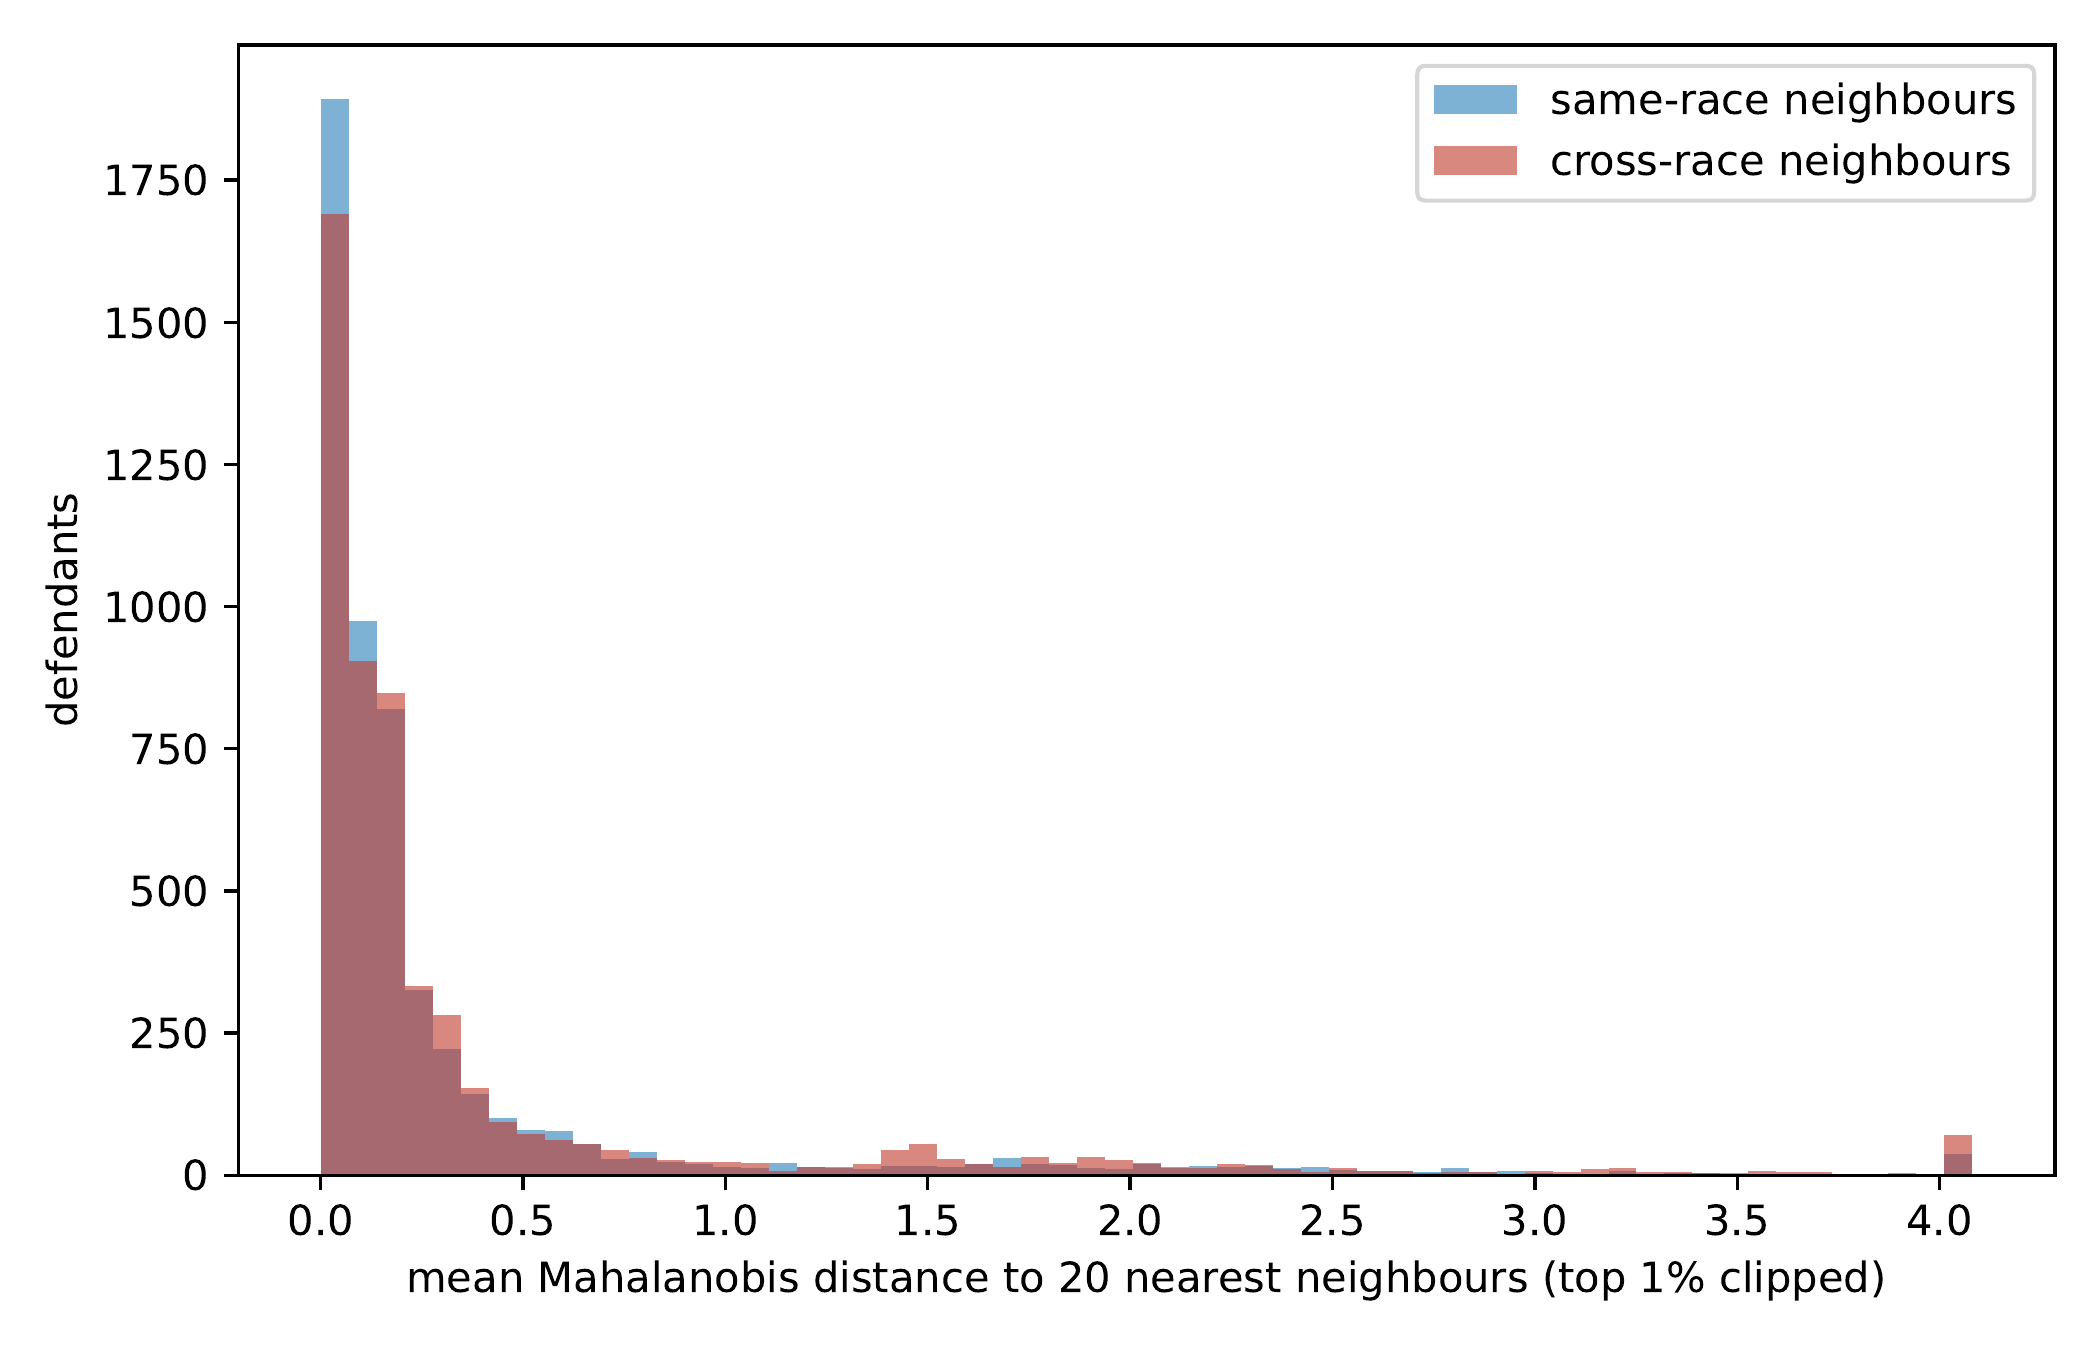
\includegraphics[width=0.75\textwidth]{figures/distance_diagnostics.pdf}
\caption{Distribution over defendants of the mean Mahalanobis
distance to the 20 nearest same-race and cross-race neighbours.
Cross-race neighbours are systematically farther (mean ratio 1.28),
which by itself can inflate LBI under a race-blind score; the
specifications of \S\ref{sec:distdiag} quantify how much.}
\label{fig:distdiag}
\end{figure}

\textbf{Matching-parity specifications.} We re-estimate
$\mathrm{LBI}(\text{race})$ at $k = 20$ under five specifications
that tighten or equalize matching quality
(Table~\ref{tab:matchparity}):

\begin{table}[h]
\centering
\caption{$\mathrm{LBI}(\text{race})$ at $k = 20$ under
matching-parity specifications. CIs for restricted specifications are
naive percentile bootstrap over per-defendant quantities and are
reported for orientation only.}
\label{tab:matchparity}
\begin{tabular}{lrrl}
\toprule
\textbf{Specification} & \textbf{LBI} & $n$ \textbf{used} & \textbf{Note} \\
\midrule
unrestricted (baseline) & 1.049 & 5{,}278 & \\
exact match on felony indicator & 1.050 & 5{,}278 & then Mahalanobis \\
caliper: cross-race NN within q90 of same-race NN & 1.022 & 4{,}656 & \\
caliper: within q75 & 1.012 & 3{,}826 & \\
fixed-radius neighbourhoods (median $k{=}20$ radius) & 1.022 & 4{,}171 & \\
coarsened-exact strata, then Mahalanobis & 1.009 & 3{,}159 & CI $[1.000, 1.018]$ \\
distance-matched same-race comparators & 1.003 & 5{,}278 & overcorrects; see text \\
\bottomrule
\end{tabular}
\end{table}

Exact matching on the felony indicator before continuous matching
changes nothing ($1.050$): the charge-degree indicator was already
well matched. The caliper analyses---excluding focal defendants whose
nearest cross-race comparator is farther than the 90th (75th)
percentile of nearest same-race distances---attenuate the index to
$1.022$ ($1.012$). Fixed-radius neighbourhoods, which force both
comparison sets inside the same ball, give $1.022$. Coarsened-exact
matching (age, priors, any-juvenile, felony bins; Mahalanobis within
stratum) gives $1.009$ $[1.000, 1.018]$ on the $3{,}159$ defendants
with sufficient within-stratum comparators. The distance-matched
specification selects, for each defendant, same-race comparators at
the same distances as the cross-race set; because the greedy matching
overshoots (mean same-race comparator distance $0.662$ vs.\
cross-race $0.458$), it \emph{overcorrects}---the same-race baseline
is drawn from strictly worse matches---and its value of $1.003$ is
best read as a lower bound.

\textbf{Where the signal lives.} The reviewer-requested distribution
of per-defendant contrasts (Figure~\ref{fig:gapdist}) completes the
picture: at $k = 20$, 53.9\,\% of defendants have a positive
cross-minus-same gap (mean $+0.108$ deciles, median $+0.100$), and
excluding the top 5\,\% of gaps lowers the index from $1.049$ to
$1.009$. The unadjusted index is thus materially driven by its upper
tail---defendants, disproportionately in the sparse high-priors
region where close cross-race comparators are scarce, whose
cross-race score divergence is large.

\begin{figure}[h]
\centering
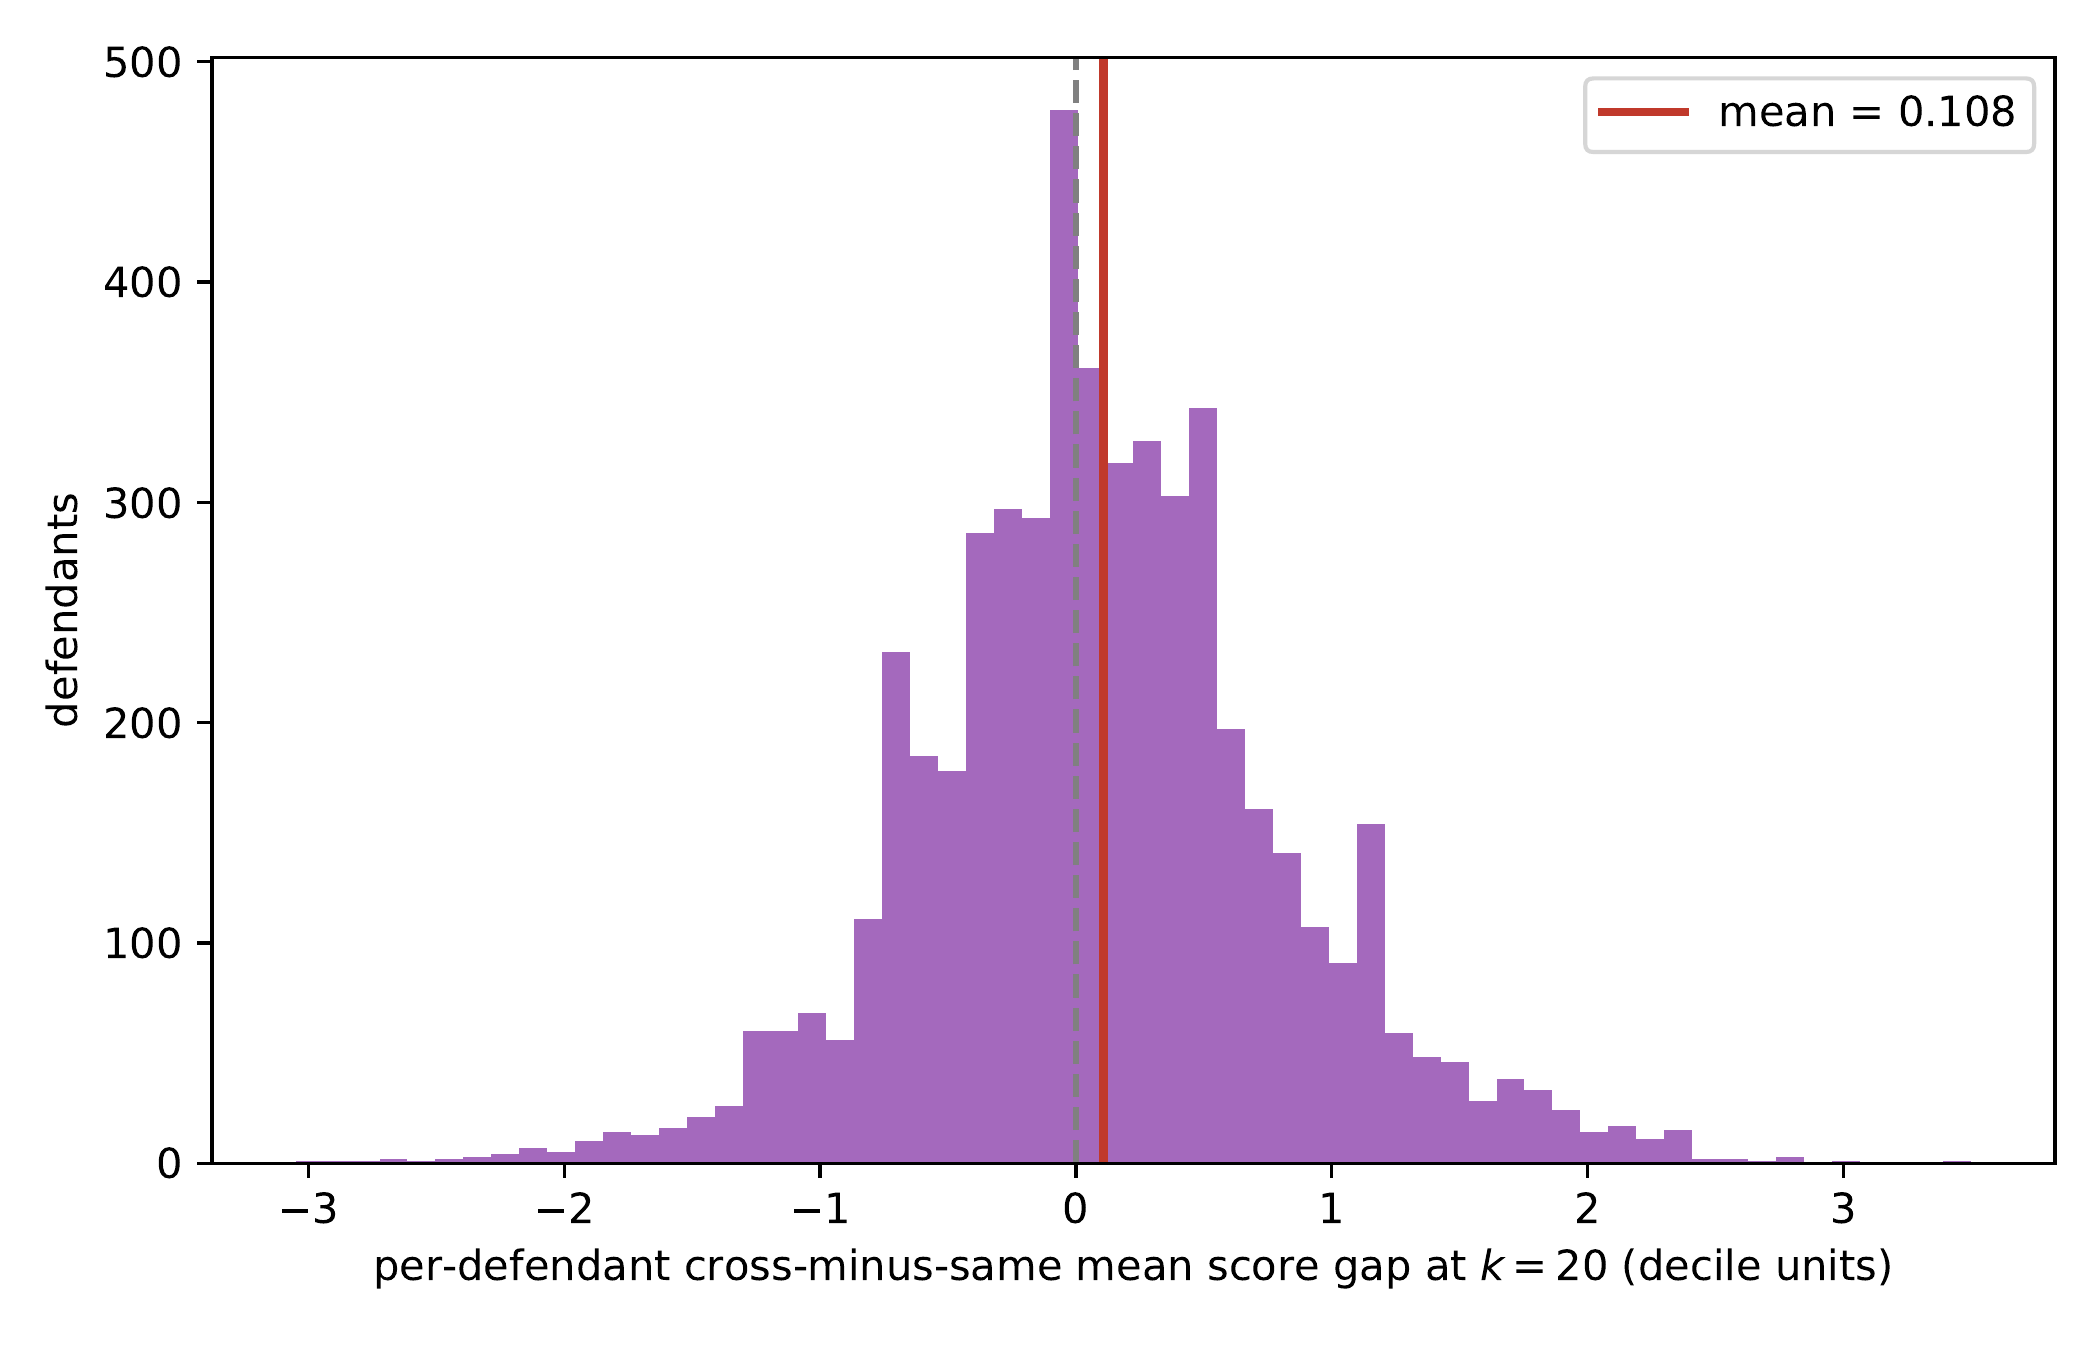
\includegraphics[width=0.75\textwidth]{figures/gap_distribution.pdf}
\caption{Distribution over defendants of the per-defendant
cross-minus-same mean score gap at $k = 20$ (decile units). The mass
is centred just above zero (53.9\,\% positive) with a heavy right
tail; excluding the top 5\,\% lowers the aggregate LBI from 1.049 to
1.009.}
\label{fig:gapdist}
\end{figure}

Taken together, the diagnostics support a two-component reading of
the unadjusted $1.049$: a mechanical component attributable to the
poorer average quality of cross-race matches (on the order of
$+0.01$ to $+0.015$; compare the race-blind synthetic level of
$1.009$ and the conditional null centre of $1.015$ in
\S\ref{sec:synthetic} and \S\ref{sec:inferenceresults}), and a
residual race-associated component that is concentrated in the
poorly-overlapped region of feature space and in the upper tail of
the gap distribution. The inferential question---is the residual
component distinguishable from zero once the mechanical component is
built into the null?---is answered next.

\subsection{Randomization inference at full sample size}
\label{sec:inferenceresults}

Table~\ref{tab:nulls} reports the three null constructions of
\S\ref{sec:inference}, each with 1{,}000 draws, with observed and
null statistics computed identically on the full $n = 5{,}278$ (the
earlier version of this paper computed the null on 500-defendant
subsamples with 200 permutations; both departures are corrected
here).

\begin{table}[h]
\centering
\caption{Null distributions for $\mathrm{LBI}(\text{race})$,
1{,}000 draws each, full sample. $z$ is the observed value ($1.049$
at $k = 20$) standardized against the null; the global $p$ uses the
max-$z$ statistic across all six scales.}
\label{tab:nulls}
\begin{tabular}{lrrrr}
\toprule
\textbf{Null construction} & \textbf{null mean} & \textbf{null SD}
 & \textbf{$z$ ($k{=}20$)} & \textbf{global $p$} \\
\midrule
plain permutation & 1.0013 & 0.0049 & 9.7 & $0.001$ \\
stratified permutation (propensity deciles) & 1.0124 & 0.0066 & 5.5 & $0.001$ \\
conditional randomization (CRT) & 1.0150 & 0.0068 & 4.9 & $0.001$ \\
\bottomrule
\end{tabular}
\end{table}

Two features deserve emphasis. First, the stricter nulls are
\emph{not} centred at $1$: preserving the race--feature dependence
shifts the null centre to $1.012$--$1.015$, which is precisely the
mechanical matching component the reviewer anticipated---a race-blind
score on these feature distributions is expected to produce an LBI of
about $1.015$, not $1.000$. The plain permutation test, whose null is
centred at $1.001$, therefore tests the wrong hypothesis, and
\S\ref{sec:synthetic} shows it false-fires on more than half of
race-blind synthetic datasets. Second, even against the correctly
centred conditional null, the observed index rejects decisively: $z
= 4.9$, pointwise and global $p = 0.001$ (no null draw's max-$z$
reached the observed), with the stratified permutation---a
nonparametric check on the CRT's logistic propensity model---agreeing
($z = 5.5$). Figure~\ref{fig:permutation} shows both nulls against
the observed value.

\begin{figure}[h]
\centering
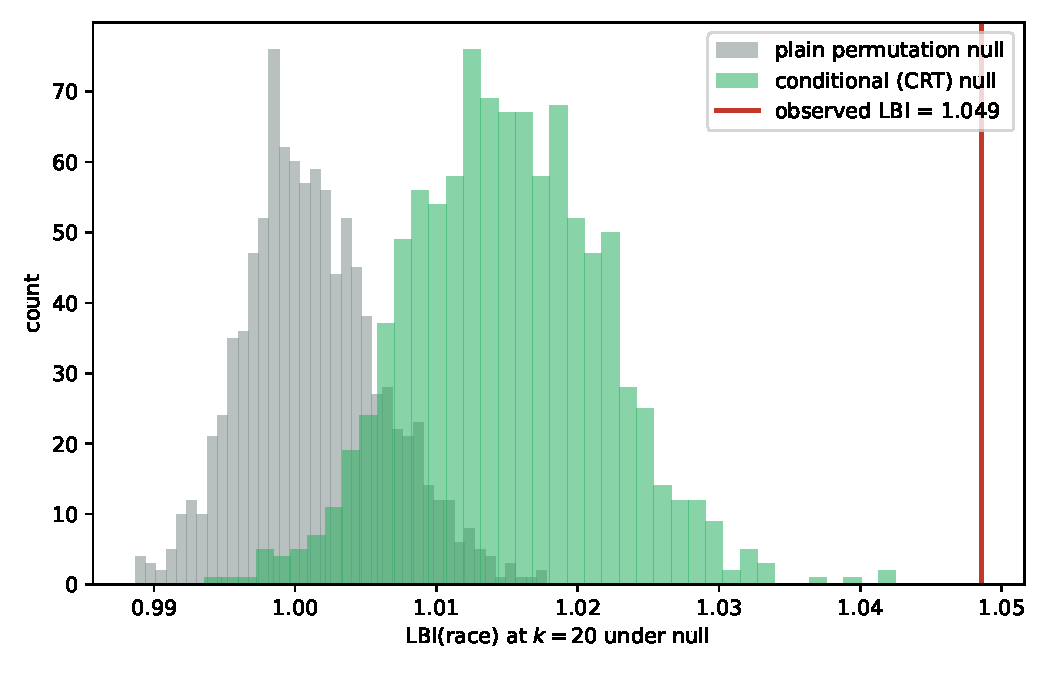
\includegraphics[width=0.75\textwidth]{figures/lbi_permutation.pdf}
\caption{Null distributions of LBI(race) at $k = 20$ from 1{,}000
draws at full sample size: plain permutation (grey) and the
conditional randomization test preserving
$\hat{P}(\text{race} \mid \mathbf{x})$ (green). The conditional null
is centred at $1.015$, not $1.000$---the mechanical component of the
index under race-blind scoring. The observed value (red line) lies
$z = 4.9$ above the conditional null; no draw exceeded it under
either construction.}
\label{fig:permutation}
\end{figure}

\subsection{Scores, categories, and classifications}
\label{sec:scorerep}

COMPAS deciles map to three published categories: 1--4 ``low,'' 5--7
``medium,'' 8--10 ``high.'' ProPublica's binary analysis treated
``medium or high'' (decile $\geq 5$) as its ``higher risk'' class;
we report that threshold under its proper name, add the $\geq 8$
(``high'' only) threshold, and caution that neither is universally
decision-relevant---operational cutoffs vary by jurisdiction and
decision point. Because a ratio alone cannot convey practical
magnitude, Table~\ref{tab:scorerep} reports the raw numerator and
denominator: the mean cross-race and same-race
classification-disagreement rates among matched neighbours.

\begin{table}[h]
\centering
\caption{$\mathrm{LBI}(\text{race})$ at $k = 20$ by score
representation, with the underlying matched-neighbour disagreement
rates (for the decile row, mean absolute score gaps in decile
units). Naive bootstrap CIs.}
\label{tab:scorerep}
\begin{tabular}{lrrrl}
\toprule
\textbf{Representation} & \textbf{LBI} & \textbf{cross rate} &
\textbf{same rate} & \textbf{95\,\% CI} \\
\midrule
raw decile (1--10) & 1.049 & 2.323 & 2.215 & $[1.039, 1.058]$ \\
three-category (low/med/high) & 1.065 & 0.619 & 0.582 & $[1.052, 1.077]$ \\
binary medium-or-high ($\geq 5$; ProPublica) & 1.092 & 0.373 & 0.342 & $[1.077, 1.106]$ \\
binary high ($\geq 8$) & 1.026 & 0.246 & 0.240 & $[1.007, 1.045]$ \\
\bottomrule
\end{tabular}
\end{table}

At ProPublica's medium-or-high threshold, matched cross-race
neighbour pairs disagree on the classification 37.3\,\% of the time
against a same-race rate of 34.2\,\%: a 3.1-percentage-point
absolute, 9.2\,\% relative excess. At the ``high'' threshold the
excess is smaller (1.026; 24.6\,\% vs.\ 24.0\,\%). The disparity is
therefore largest exactly at the cutoff that drove the public
controversy, and an LBI of 1.092 should be read as a 9.2\,\%
\emph{relative} increase in disagreement, not a nine-point one.

\subsection{Robustness: feature sets and matching methods}
\label{sec:robustness}

The standing objection to any matched-comparison diagnostic is that
the signal is an artefact of the analyst's choices: the feature list,
or the matching machinery itself. Table~\ref{tab:robust} tests both.
(All rows use the rebuilt pipeline with deterministic tie-breaking;
naive bootstrap CIs.)

\begin{table}[h]
\centering
\caption{Robustness of $\mathrm{LBI}(\text{race})$ at $k = 20$.
Top: legitimate-feature set (Mahalanobis, decile score). Bottom:
matching method (six features, decile score).}
\label{tab:robust}
\begin{tabular}{lrl}
\toprule
\textbf{Specification} & \textbf{LBI} & \textbf{95\,\% CI} \\
\midrule
\multicolumn{3}{l}{\emph{Feature set}}\\
\quad minimal (age, priors) & 1.034 & $[1.025, 1.042]$ \\
\quad paper (6 features) & 1.049 & $[1.039, 1.058]$ \\
\quad drop contested juvenile counts & 1.034 & $[1.025, 1.042]$ \\
\quad paper $+$ sex control\textsuperscript{$\dagger$} & 1.060 & $[1.050, 1.071]$ \\
\midrule
\multicolumn{3}{l}{\emph{Matching method}}\\
\quad Euclidean on standardized features & 1.048 & $[1.038, 1.057]$ \\
\quad robust Mahalanobis (MinCovDet) & 1.048 & $[1.039, 1.057]$ \\
\quad $\log(1{+}x)$ on count features, Mahalanobis & 1.048 & $[1.038, 1.057]$ \\
\quad rank transform, Euclidean & 1.044 & $[1.035, 1.053]$ \\
\quad Gower distance (mixed-type) & 1.049 & $[1.040, 1.059]$ \\
\bottomrule
\end{tabular}

\smallskip
{\footnotesize \textsuperscript{$\dagger$}Adding sex as a matching
control \emph{raises} the race index (1.049 $\to$ 1.060) because
within-sex matching removes cross-sex dilution: without the control,
some matched neighbours differ in sex as well as race, and averaging
over those pairs attenuates the race-specific gap.}
\end{table}

The unrestricted index is insensitive to both choices: every feature
set yields $\mathrm{LBI} \geq 1.034$ with CIs excluding 1---including
the specification that \emph{drops} the racially patterned juvenile
counts---and the five alternative distance constructions agree to
within $0.005$. (The matching-\emph{parity} restrictions of
\S\ref{sec:distdiag} are the specifications that move the estimate;
robustness to the metric family is not the same as robustness to
match quality, and the two should not be conflated.) The deeper
omitted-variable concern---COMPAS inputs absent from the public file
(substance use, education, employment) cannot be matched on---remains,
and is exactly the failure mode quantified as condition 4 of the
synthetic validation below.

\subsection{Validation under known ground truth}
\label{sec:synthetic}

A new diagnostic should demonstrate what it detects. We build
semi-synthetic scores on the \emph{real} feature matrix and race
labels---preserving the actual race--feature dependence---and run the
full pipeline (estimator plus tests) under four known conditions. The
base score is $\hat{f}_0(\mathbf{x})$, a linear fit of the observed
decile on the six standardized features ($R^2 = 0.42$, residual SD
$\sigma = 2.16$ deciles), plus Gaussian noise of the same residual
scale. Conditions: (1) \emph{race-blind}: $S = \hat{f}_0(\mathbf{x})
+ \varepsilon$; (2) \emph{direct}: add $\beta \cdot
\mathbf{1}[\text{Black}]$ for $\beta \in \{0.25, 0.5, 1.0\}$ deciles;
(3) \emph{proxy}: add $\gamma Z$ where $Z$ has correlation $0.8$
with race and $\gamma \in \{0.5, 1.0\}$; (4) \emph{omitted
legitimate predictor}: race-blind score built on all six features,
matching on only five (priors count withheld). Each condition runs
$60$--$200$ Monte Carlo replicates; each replicate is tested at the
5\,\% level by plain permutation and by CRT (200 draws each), with an
OLS race-coefficient $t$-test as a parametric baseline.

\begin{table}[h]
\centering
\caption{Semi-synthetic validation at $k = 20$. ``Reject \%'' is the
fraction of replicates in which each test rejects at the nominal
5\,\% level: under condition 1 this is the false-positive rate;
under conditions 2--3, power. The Dwork-style nearest-neighbour
consistency of the last column is flat across the race-structure
conditions (1--3) and responds only to the omitted-predictor
condition, illustrating that it measures smoothness of the score in
the matching space, not protected-attribute structure.}
\label{tab:synthetic}
\begin{tabular}{lrrrrr}
\toprule
\textbf{Condition} & \textbf{mean LBI} &
\multicolumn{3}{c}{\textbf{Reject \% (5\,\% level)}} &
\textbf{consistency} \\
\cmidrule(lr){3-5}
 & & perm & CRT & OLS & \\
\midrule
1.\ race-blind & $1.009 \pm 0.006$ & 56.5 & 4.5 & 6.0 & 0.37 \\
2.\ direct, $\beta = 0.25$ & $1.015 \pm 0.006$ & 88.3 & 21.7 & 100 & 0.37 \\
2.\ direct, $\beta = 0.5$ & $1.027 \pm 0.007$ & 100 & 85.0 & 100 & 0.37 \\
2.\ direct, $\beta = 1.0$ & $1.071 \pm 0.010$ & 100 & 100 & 100 & 0.38 \\
3.\ proxy, $\gamma = 0.5$ & $1.052 \pm 0.008$ & 100 & 100 & 100 & 0.38 \\
3.\ proxy, $\gamma = 1.0$ & $1.153 \pm 0.013$ & 100 & 100 & 100 & 0.37 \\
4.\ omitted predictor & $1.015 \pm 0.006$ & 88.3 & 5.0 & 1.7 & 0.31 \\
\bottomrule
\end{tabular}
\end{table}

Table~\ref{tab:synthetic} and Figure~\ref{fig:synthetic} deliver five
conclusions.

\begin{enumerate}[leftmargin=*]
\item \emph{Under a race-blind score the index sits near---but not
at---1} ($1.009 \pm 0.006$): the mechanical matching component of
\S\ref{sec:distdiag} is real but small on these data.
\item \emph{The plain permutation test is badly anticonservative}
(false-positive rate 56\,\% at the nominal 5\,\% level), confirming
quantitatively the concern raised in review; it should not be used
with LBI, and we retain it only as a cautionary row. The CRT is
correctly calibrated (4\,\%).
\item \emph{The index rises monotonically with direct
discrimination} ($1.009 \to 1.015 \to 1.027 \to 1.071$ as $\beta$
runs $0 \to 1$ decile) and responds strongly to proxy discrimination
($1.153$ at $\gamma = 1$), which a race-blind-inputs audit would
miss entirely.
\item \emph{Matching failure inflates the point estimate but not the
calibrated test}: withholding a legitimate predictor from the
matching set (condition 4) raises mean LBI to $1.015$, yet the CRT
still rejects at only 5\,\%---because the CRT conditions on the full
covariate set, its validity survives an impoverished matching space,
provided the audit \emph{records} the covariate even when it cannot
match well on it. When a legitimate determinant is unrecorded, both
LBI and every other observational diagnostic inherit the bias; that
is the irreducible limitation of \S\ref{sec:discussion}.
\item \emph{Comparators}: the OLS race coefficient is more powerful
than LBI against purely linear direct effects (100\,\% vs.\ 21.7\,\%
at $\beta = 0.25$)---parametric tests win on their home turf---while a
Dwork-style nearest-neighbour consistency score is flat across the
race-structure conditions (0.37--0.38 as the injected effect grows
from zero to its largest value) and moves only when a legitimate
predictor is withheld from the matching space (0.31 under condition
4), confirming that it measures smoothness of the score in the
matched coordinates, not protected-attribute structure. LBI's role is
the model-free middle
ground: no functional-form assumption, black-box outputs (including
purely categorical ones), and a null-calibrated test.
\end{enumerate}

\begin{figure}[h]
\centering
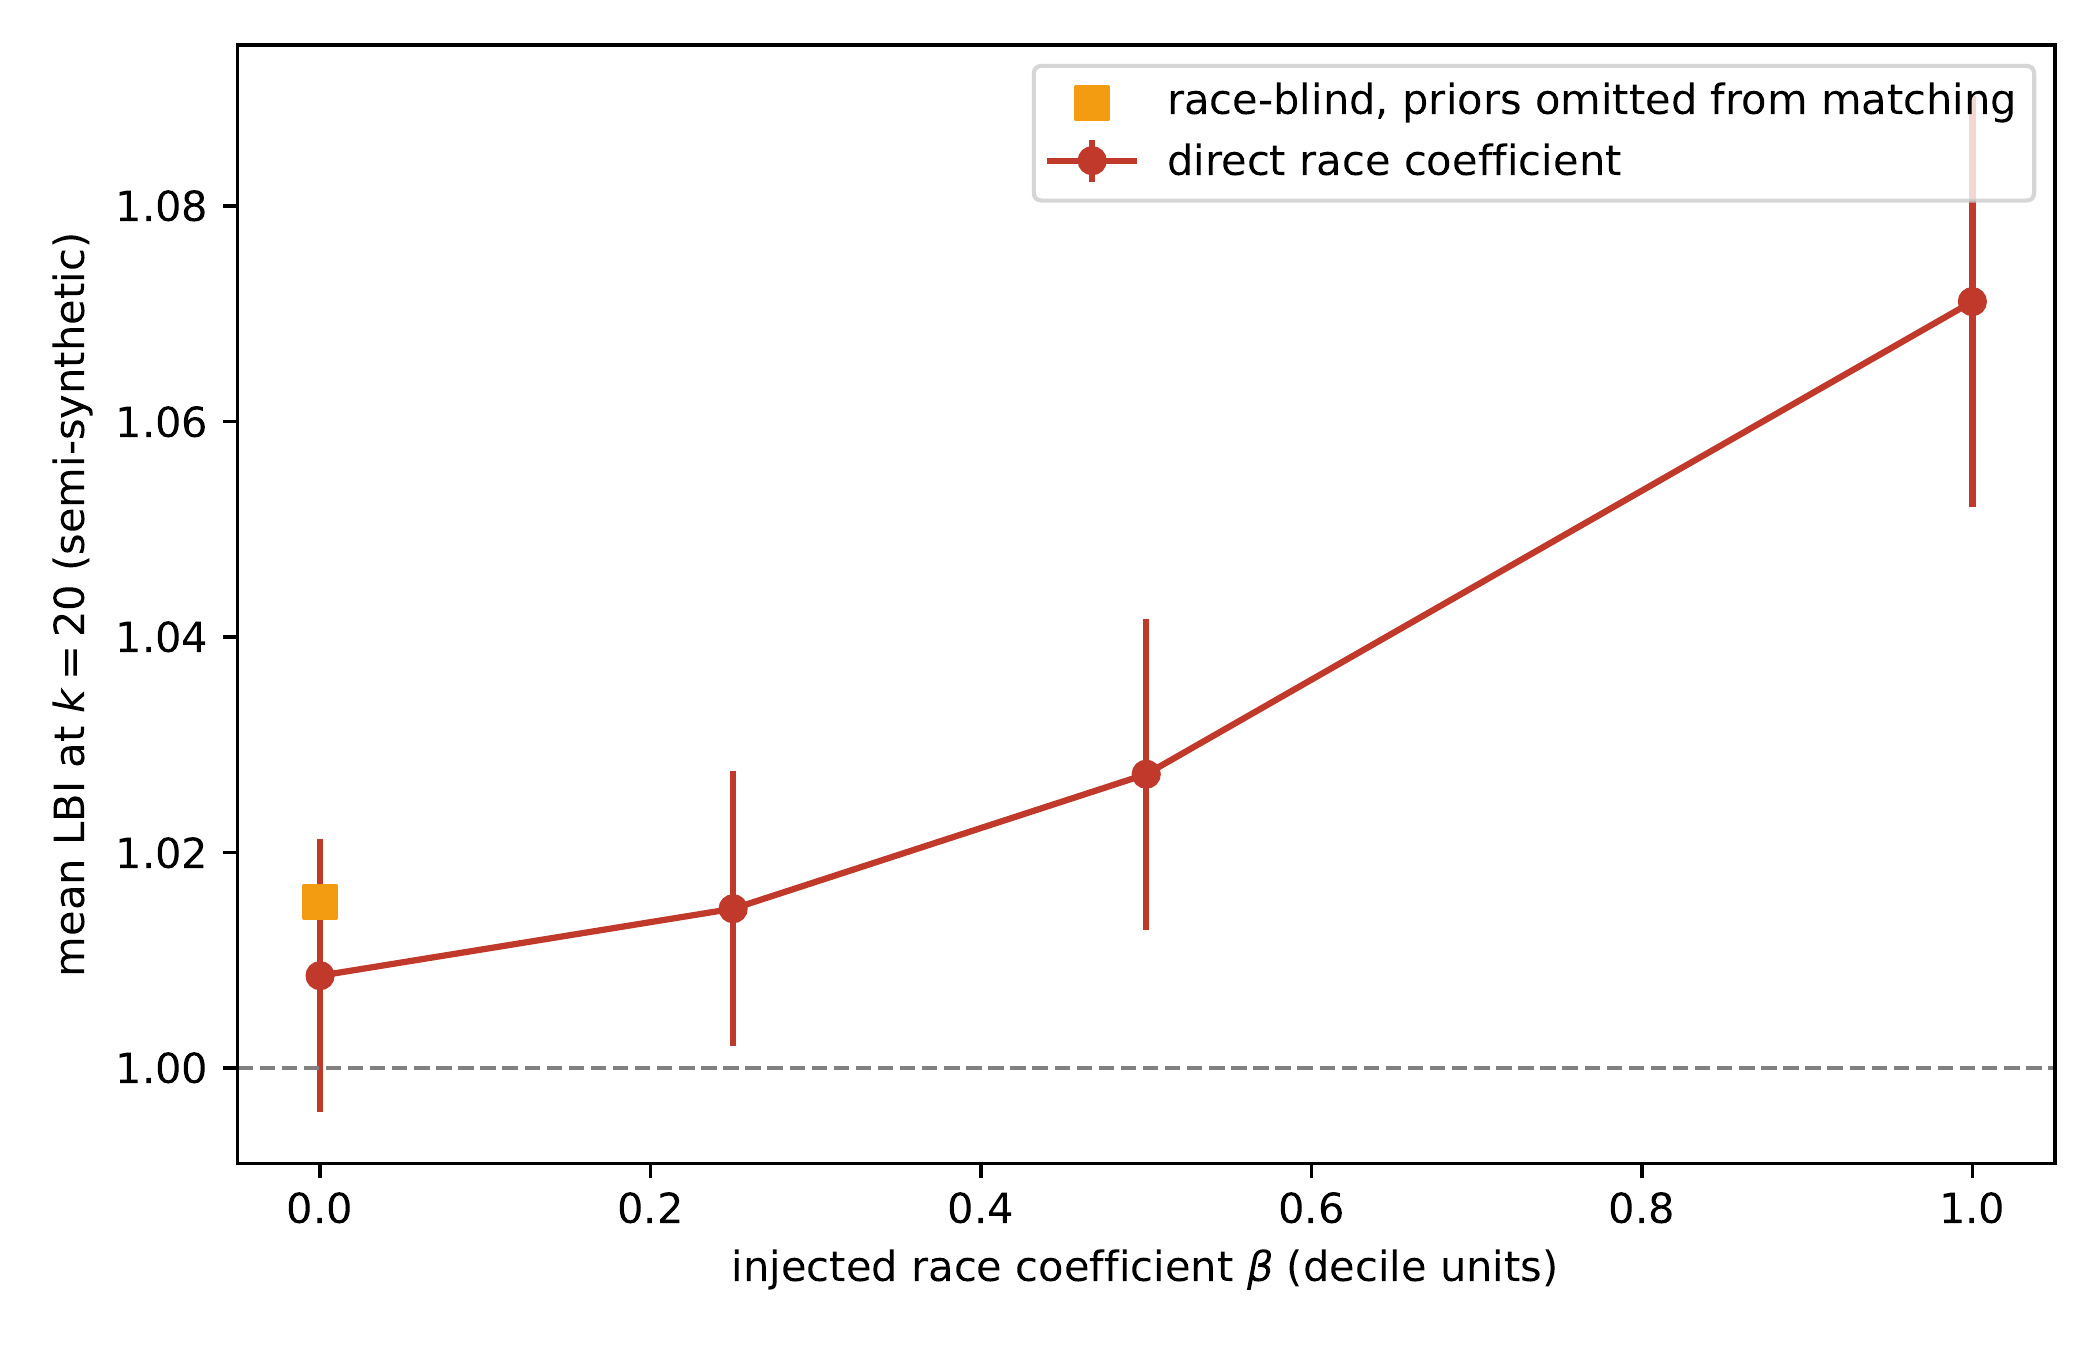
\includegraphics[width=0.75\textwidth]{figures/synthetic_validation.pdf}
\caption{Semi-synthetic validation: mean LBI at $k = 20$ (error bars
$\pm 2$ SD over replicates) as a function of an injected direct race
coefficient $\beta$, on the real COMPAS feature distributions. The
race-blind level is $1.009$, not $1.000$ (the mechanical matching
component); the response is monotone in $\beta$. The orange square
marks condition 4 (race-blind score, priors count omitted from the
matching set), whose inflation to $1.015$ quantifies the
matching-failure failure mode.}
\label{fig:synthetic}
\end{figure}

\subsection{Implementation details}
\label{sec:implementation}

For audit reproducibility we record the implementation choices that
the review process surfaced as material. \emph{Ties and duplicates}:
the six-feature space is heavily duplicated---3{,}673 of 5{,}278
defendants share their exact feature vector with at least one
other---so distance ties are pervasive (79\,\% of defendants have a
tie straddling the $k = 20$ neighbourhood boundary). Neighbour
selection uses a stable sort, so tie-breaking is deterministic (by
dataset row order); estimates at $k = 1$ are the most tie-sensitive,
which is why small-$k$ values should be read with their (wide) CIs.
\emph{Score ties} raise no issue: score gaps enter as absolute
differences. \emph{Neighbour reuse}: each defendant appears in a mean
of 40 (max 198) other defendants' comparison sets; the
re-formed-neighbourhood bootstrap propagates this dependence into the
CIs. \emph{Missing values}: none among the six features in the
filtered subset. \emph{Covariance inversion}: the correlation matrix
has condition number 2.65; inversion uses a ridge of $10^{-6}$.
\emph{Insufficient comparators}: in unrestricted analyses every
defendant has at least $k = 100$ comparators of each group; under
exact-stratum and coarsened-exact restrictions, defendants lacking
$k$ within-stratum comparators of either group are excluded and the
retained $n$ is reported alongside the estimate.

\subsection{Summary}

Table~\ref{tab:summary} summarizes the empirical findings.

\begin{table}[h]
\centering
\caption{Headline fairness measurements on the COMPAS Black/White
subset, $n = 5{,}278$.}
\label{tab:summary}
\begin{tabular}{p{0.53\textwidth}lp{0.34\textwidth}}
\toprule
\textbf{Metric} & \textbf{Value} & \textbf{Interpretation} \\
\midrule
Disparate impact (Black/White, medium-or-high) & $1.741$ &
Fails the four-fifths screen if translated from employment law
(illustrative only; \S\ref{sec:doctrine}) \\
FPR disparity (Black $-$ White) & $+0.203$ &
ProPublica's headline finding; large \\
FNR disparity (Black $-$ White) & $-0.211$ &
Complementary rate (distinct denominator); large \\
Predictive-parity gap, $\Pr(\text{recid}\mid\text{high})$ (Black $-$ White) & $+0.055$ &
Northpointe's defence; small \\
\midrule
\textbf{LBI(race) at $k = 20$} & $\mathbf{1.049}$ &
\textbf{CI $[1.027, 1.072]$; CRT $z = 4.9$, global $p = 0.001$} \\
\quad under matching-parity restrictions & $1.00$--$1.02$ &
mechanical component removed (\S\ref{sec:distdiag}) \\
\quad at the medium-or-high threshold & $1.092$ &
disagreement rates 37.3\,\% vs.\ 34.2\,\% \\
\bottomrule
\end{tabular}
\end{table}

The honest summary is two-sided. The unadjusted index overstates the
race-associated component: roughly $+0.01$ to $+0.015$ of the excess
is mechanical, attributable to cross-race neighbours being
worse-matched on these feature distributions, and specifications
that force matching parity land at $1.01$--$1.02$. What remains is
nonetheless statistically unambiguous under the correctly calibrated
conditional test ($z = 4.9$, global $p = 0.001$ across all scales),
is concentrated among defendants with scarce cross-race comparators
and in the upper tail of the gap distribution, is asymmetric across
focal groups ($1.087$ White-focal vs.\ $1.027$ Black-focal), and is
largest at the classification threshold that drove the public
controversy ($1.092$; 37.3\,\% vs.\ 34.2\,\% disagreement).


%==============================================================================
\section{Discussion}
\label{sec:discussion}
%==============================================================================

\subsection{What LBI adds to the fairness literature}

LBI complements rather than replaces the existing fairness metrics.
Three properties distinguish it:

\textbf{(i) It is matched-neighbourhood, not marginal.} The
Chouldechova--Kleinberg impossibility is a constraint on marginal,
group-level statistics (error rates and calibration conditioned only
on group and outcome). LBI is built from local comparisons between
defendants matched on legitimate predictors and then aggregated, so
it is best described as a population-level summary of case-level
contrasts; what distinguishes it from the marginal metrics is the
\emph{conditioning}---every comparison is between similarly-situated
defendants---not the level of aggregation. The impossibility theorem
does not constrain it: an algorithm can have $\mathrm{LBI} = 1$
without satisfying either calibration or equalized odds, and
conversely.

\textbf{(ii) It is a compact, reportable object.} Population-level
metrics typically come in matched pairs (FPR and FNR; precision at
high and low; positive-prediction rate by group). LBI is a
scale-indexed curve with pointwise confidence intervals and a single
global test, a compact form that could slot into audit-style
reporting if the metric matures beyond its current research stage.
Compactness is a reporting convenience, not an epistemic virtue:
case-level disparity may itself vary by offence type, decision point,
or assessment window---and on COMPAS it demonstrably varies by focal
group and by region of feature space (\S\ref{sec:lbiresults},
\S\ref{sec:distdiag})---so the index is best read as a screening
signal to be disaggregated when it fires, not a substitute for the
fuller metric panel.

\textbf{(iii) It depends on a metric on legitimate predictors, not
on the algorithm's internals.} LBI can be computed by an auditor
who has access to the inputs and outputs of the algorithm but not
to its parameters. This is the typical audit setting: a regulator
or oversight body can observe predictions but not the model.

\subsection{Relationship to individual fairness}
\label{sec:individualfairness}

\citet{dwork2012} introduced individual fairness as the requirement
that ``similar individuals are treated similarly,''
formalized as a Lipschitz constraint with respect to a
task-appropriate metric. They acknowledged the difficulty of
specifying the metric and treated it as an open problem.

LBI is not an implementation of individual fairness; it is a
matched-neighbourhood disparity diagnostic \emph{inspired by}
individual-fairness principles, with two specific choices: the
metric is the Mahalanobis distance on the available legitimate
predictors, and the quantity reported is the matched-pair $k$-NN
ratio rather than a uniform Lipschitz bound. The distinction
matters, and it is a weakness of the approach relative to the ideal:
because the matching metric is defined only on the \emph{measured}
predictors---a subset of what COMPAS uses---matched neighbours are
similar in the measured coordinates, not certifiably similar
simpliciter, so LBI can neither verify nor refute the
Dwork-style property itself. What the matched-pair formulation buys
is operational tractability---to verify a uniform Lipschitz bound,
one must evaluate the algorithm on all pairs in the domain, which is
infeasible for any non-trivial population---at the price of this
weaker, conditional guarantee.

\subsection{Relationship to counterfactual fairness}

\citet{kusner2017} require that the algorithm's output be invariant
under a counterfactual change of the protected attribute, holding
the legitimate features fixed at their observed values. This is a
strict version of case-level fairness; LBI is a soft version. The
strict version requires a causal model of how the legitimate
features depend on the protected attribute; the soft version (LBI)
does not. The relationship between the two is heuristic, not exact,
because LBI compares \emph{different individuals} while
counterfactual fairness compares counterfactual versions of the
\emph{same} individual: if the matching features capture all
legitimate determinants of the score and matched neighbours are
close, a counterfactually fair algorithm will exhibit
$\mathrm{LBI} \approx 1$; and an elevated LBI is what counterfactual
unfairness would produce, but it can also be produced by omitted
legitimate determinants (\S\ref{sec:synthetic}, condition 4), so the
implication runs cleanly only in the presence of a causal model.

\subsection{Limitations}

\textbf{Choice of legitimate features, and contested proxies.} The LBI
signal depends on what we declare ``legitimate,'' and that choice is
normative, not merely practical---data availability cannot substitute for
legal justification. Two failure modes cut in opposite directions. If
relevant legitimate predictors are \emph{omitted}, matched pairs are not
truly similarly situated and LBI can \emph{overstate} unfairness; the
public ProPublica file omits COMPAS inputs such as substance-use,
education, and employment items, so our matching is necessarily on a
subset. Conversely, some included features are themselves
\emph{racially patterned proxies}---prior counts and juvenile counts
reflect policing, surveillance, and charging practices as much as
underlying conduct---so controlling on them can \emph{understate}
unfairness by normalizing part of the very disparity we seek to measure.
These features are therefore not ``uncontroversial''; a careful audit
distinguishes predictors that are legitimate-and-available,
legitimate-but-unavailable, and available-but-contested. The robustness
analysis (\S\ref{sec:robustness}) shows the case-level signal survives
every available-feature choice we can test---including \emph{dropping}
the contested juvenile counts---but the unmeasured COMPAS inputs remain a
genuine limit on any claim of complete case-level similarity. To state
the weakness plainly: because the public dataset contains only a subset
of the variables COMPAS uses, this analysis cannot establish full
individual fairness or its violation---it cannot confirm that the
compared defendants were fully similarly situated, cannot isolate a
causal effect of race, and cannot prove discrimination. Every finding
in this paper is conditional on the measured predictors.

\textbf{External validity of the semi-synthetic validation.} The
validation suite of \S\ref{sec:synthetic} is built on the COMPAS
feature matrix, its race--feature dependence, and one linear score
family. It establishes calibration and power \emph{in this setting};
it does not establish that the metric or its inference machinery will
perform consistently across other algorithms, jurisdictions, or
decision settings. This is a weakness of the present evidence:
transportability of the diagnostic is untested, and each new setting
requires its own ground-truth validation before the index is relied
upon there.

\textbf{Binary protected attributes.} Definition~\ref{def:lbi} treats
the protected attribute as binary. Multi-class extension is
straightforward in either of two ways: compute pairwise LBI between
all pairs of classes (giving a matrix of values), or take a
one-vs-rest formulation. The COMPAS analysis uses the
African-American vs.\ Caucasian binary because that is the contrast
that drove the public controversy; the extension to multiple race
categories is mechanical.

\textbf{The 5\,\% magnitude.} The COMPAS LBI of $1.049$ is
statistically robust but quantitatively modest, and because it is a
\emph{relative} measure, its practical import depends on the
underlying rates: at the binary medium-or-high threshold, the
matched cross-race classification-disagreement rate is
37.3\,\% against a same-race rate of 34.2\,\%---a
9.2\,\% relative excess, or 3.1 percentage points
(\S\ref{sec:scorerep}). The legal and regulatory significance of an
excess of this size is a policy question, not a statistical one; and
the matching-parity analyses of \S\ref{sec:distdiag} imply the
adjusted excess on the decile score is smaller still
($1.00$--$1.02$).

\textbf{Mahalanobis on $\mathbb{R}^d$.} For continuous and binary
features the Mahalanobis metric is well-defined; for genuinely
categorical features (e.g., charge type with twenty levels), a
modified metric (Gower distance, learned similarity, propensity
score) may be more appropriate. The COMPAS feature space is
predominantly continuous so this issue does not arise here. In
settings where cases are unstructured documents rather than feature
vectors, a learned case-similarity embedding could in principle
supply the metric, but it should not be assumed adequate:
general-purpose text embeddings conflate legal structure with
generic textual similarity, so any learned metric should be
validated against external structure (citation networks, expert
similarity judgments) before it anchors a fairness audit. The
metric is a substantive, validated input to the audit, not a
commodity.

\textbf{Causal disentanglement.} LBI measures a statistical
association between the protected attribute and the algorithm's
output, controlling for legitimate features via the Mahalanobis
neighbourhood. It does not by itself establish a causal mechanism
for that association. The causal story may be that the algorithm
encodes race indirectly through correlated features that are not
in our legitimate-feature set (residential zip code, employment
history). Distinguishing these causal pathways is beyond what LBI
alone can do; LBI is an audit signal that flags the issue and
quantifies its magnitude, not a complete causal account.


%==============================================================================
\section{Policy and Regulatory Implications}
\label{sec:policy}
%==============================================================================

\subsection{A research-stage screening signal for legal-AI audits}

The LBI is a research-stage screening signal that may contribute one
input to an audit of a scored or classified decision process; it is
not a validated regulatory audit standard, and nothing in this paper
should be read as certifying it for that role. Its validation to date
consists of one dataset and one semi-synthetic suite
(\S\ref{sec:synthetic}), which---as noted in
\S\ref{sec:discussion}---does not establish consistent performance
across other algorithms, jurisdictions, or decision settings. With
that standing caveat, the ingredients an LBI screen requires are
modest: a dataset containing the algorithm's legitimate inputs, its
outputs, and the protected attribute; the algorithm itself need not
take the protected attribute as an input---COMPAS, whose
questionnaire does not ask race, is the case in point. The candidate
procedure is:

\begin{enumerate}[leftmargin=*]
\item Obtain a sample of the algorithm's inputs and outputs, joined
to the protected attribute from administrative records ($n$ in the
thousands; the COMPAS analysis used $n = 5{,}278$).
\item Specify the legitimate-feature set (this is the normative input
that the audit cannot supply; it must come from statute,
regulation, or expert designation).
\item Compute LBI(protected attribute) across prespecified
neighbourhood scales $k$, with the matching-quality diagnostics of
\S\ref{sec:distdiag}.
\item Report the $k$-curve, pointwise confidence intervals, the
global multiscale randomization $p$-value, and the underlying
cross- and same-group rates at the operational decision threshold.
\end{enumerate}

The procedure does not require access to the algorithm's parameters,
training data, or vendor documentation. It treats the algorithm as a
black box and audits its outputs directly. This makes it well-suited
to settings where the algorithm is proprietary, as COMPAS is. The
COMPAS analysis of this paper also illustrates the procedure's
standing weakness: whatever the screen reports is conditional on the
predictors the audit dataset actually contains. Where those are a
subset of the instrument's true inputs---as here---an elevated index
does not establish that fully similarly situated individuals were
treated differently, and a null result does not certify that they
were not.
Nothing in the construction is specific to criminal justice: the same
audit applies wherever a scored or classified decision process can be
joined to legitimate features and a protected attribute---consistency
of content-moderation decisions across the identity groups mentioned
in the content, lending decisions across applicant demographics,
triage scores across patient groups---with the legitimate-feature
designation supplied, in each domain, by the governing normative
framework.

\subsection{Threshold setting}

A regulatory threshold for LBI must come from policy, not statistics,
and we propose none here. Earlier drafts of this paper offered
descriptive ranges (``probably acceptable,'' ``probably warrants
mitigation''); we have removed them, because no empirical benchmark,
power analysis, or regulatory consensus yet exists that would ground
such judgments. What can be said now is narrower and better
supported: the synthetic validation of \S\ref{sec:synthetic} shows
how the index behaves under known race-blind, direct-coefficient,
and proxy-coefficient conditions on realistic feature distributions,
and audits of this kind---accumulated across instruments and
jurisdictions---are the raw material from which defensible reference
ranges could eventually be built. Until then, an elevated LBI should
be read as a trigger for the disaggregated follow-up analyses
described above, weighed alongside the standard metric panel, not
against a numeric cutoff.

\subsection{Doctrinal context}
\label{sec:doctrine}

LBI is not a substitute for the constitutional and statutory
analysis that determines whether an algorithm's deployment is
lawful, and the doctrinal landscape it feeds into is more demanding
than a statistical disparity. Four points situate the tool.

\emph{Equal protection.} Under \emph{Washington v.\ Davis}, 426 U.S.
229 (1976), a facially neutral practice violates the Equal Protection
Clause only on a showing of discriminatory \emph{purpose}; disparate
impact alone is insufficient. \emph{McCleskey v.\ Kemp}, 481 U.S. 279
(1987), rejected an equal-protection challenge to capital sentencing
built on rigorous statistical evidence of race-correlated outcomes,
requiring proof of discriminatory purpose in the individual case. An
elevated LBI is therefore evidence of a race-associated disparity
among similarly-situated defendants---probative, perhaps, of how an
instrument operates, but nowhere near sufficient for a
constitutional claim \citep{huq2019}.

\emph{Due process and contestability.} In \emph{State v.\ Loomis},
881 N.W.2d 749 (Wis.\ 2016), \emph{cert.\ denied}, 137 S.\ Ct.\ 2290
(2017), the Wisconsin Supreme Court upheld the sentencing use of
COMPAS against a due-process challenge grounded in the instrument's
proprietary, non-inspectable methodology, while requiring written
warnings about, inter alia, undisclosed methodology and studies
questioning accuracy across racial groups. The black-box audit
posture of LBI is designed for exactly this setting: it gives courts,
defendants, and oversight bodies a quantitative handle on a
proprietary instrument's behaviour without access to its internals,
addressing part of the contestability deficit identified in the
technological due-process literature \citep{citron2008}.

\emph{Statutory frameworks.} Title VII's disparate-impact framework
(with the EEOC four-fifths heuristic) governs employment selection,
not pretrial or sentencing risk assessment; no analogous federal
statutory regime currently governs criminal-justice risk
instruments. Analyses that import the four-fifths rule into this
setting (including, descriptively, our Table~\ref{tab:summary})
should be read as illustrative translation, not doctrine.

\emph{The use of protected attributes in risk assessment.} Whether a
protected attribute is ``legally irrelevant'' is attribute- and
context-specific. Express use of race in sentencing risk assessment
is constitutionally foreclosed; sex is different---\emph{Loomis}
itself upheld COMPAS's use of sex as statistically necessary, and
some jurisdictions use sex-specific instruments---which is why we
report LBI(sex) as a comparison, not as a violation. The broader
scholarly debate on whether risk assessment can be race-neutral at
all, given racially patterned inputs like criminal history, is
developed in \citet{starr2014}, \citet{mayson2019}, and
\citet{huq2019}; our treatment of prior and juvenile counts as
``available-but-contested'' matching features
(\S\ref{sec:discussion}) follows that literature.

A high LBI does not, by itself, establish a violation of any
specific legal rule; a low LBI does not, by itself, license
deployment. LBI provides a quantitative input to legal analysis; the
legal analysis itself proceeds under the doctrinal categories
appropriate to the deployment context.


%==============================================================================
\section{Conclusion}
\label{sec:conclusion}
%==============================================================================

The COMPAS controversy crystallized a structural ambiguity in
algorithmic fairness: when group base rates differ,
no scoring rule can simultaneously satisfy calibration and equalized
error rates. The literature has responded by proliferating fairness
criteria, each capturing a different facet, none of them dispositive.

We have introduced the Legal Bond Index, a measure that sits on a
distinct axis: it summarizes matched-neighbourhood behaviour rather
than constraining marginal group statistics. On the ProPublica COMPAS
dataset the index curve lies above 1 at every prespecified
neighbourhood scale ($1.041$--$1.069$; $1.049$ at $k = 20$, 95\,\% CI
$[1.027, 1.072]$), and the finding survives the strictest inference
we could construct---a conditional randomization test whose null
absorbs the mechanical effect of cross-race neighbours being
worse-matched, validated for calibration on semi-synthetic ground
truth ($z = 4.9$, global multiscale $p = 0.001$). The same
diagnostics that certify the signal also bound it: matching-parity
specifications put the adjusted decile-score excess at $1.00$--$1.02$,
the disparity concentrates where close cross-race comparators are
scarce, and it is largest at ProPublica's medium-or-high
classification threshold ($1.092$; disagreement rates 37.3\,\% vs.\
34.2\,\%). The result is small in magnitude, statistically
unambiguous, orthogonal to the calibration--equalized-odds debate,
and reported with the diagnostics a reader needs to weigh it.

Two weaknesses bound what these findings can support, and we restate
them here so no reader overlooks them. First, the public dataset
contains only a subset of the variables COMPAS uses, so the findings
are conditional on the measured predictors: they do not establish
that fully similarly situated defendants were treated differently,
do not isolate a causal effect of race, and do not prove
discrimination. Second, the semi-synthetic validation is specific to
this dataset and score family; it does not establish that the metric
will perform consistently across other algorithms, jurisdictions, or
decision settings.

Within those limits, LBI is a matched-neighbourhood disparity
diagnostic inspired by individual-fairness principles and by
Aristotle's like-cases-alike criterion; it is cheap to compute; it
requires only an audit dataset of inputs, outputs, and the protected
attribute; and it produces a scale-indexed curve with confidence
intervals. It is offered as a research-stage screening signal that
may contribute one input to an audit, not as a validated regulatory
audit standard.

The reference implementation is openly archived on Zenodo at
\href{https://doi.org/10.5281/zenodo.21310251}{doi:10.5281/zenodo.21310251}
(concept DOI, resolving to the latest version; source in the
\texttt{ahb-sjsu/erisml-lib} repository under
\texttt{docs/papers/foundations/submission/jscilaw/}). The data, the
filter, the metric, and the figures are all reproducible from the public
ProPublica file.

\bigskip
\noindent\textbf{Author note.} LBI was originally motivated by a
geometric framework for legal analysis (the ``Judicial Complex,''
in which legal states form a weighted simplicial complex and legal
judgments are required to be invariant under legally irrelevant
transformations of the case description), developed in companion
theoretical work \citep{bond2026geometric,bond2026tractability}. The
present paper is self-contained and makes no use of that machinery;
readers interested only in LBI as an audit tool may ignore it
entirely.

\bigskip
\noindent\textbf{Data availability.} The COMPAS data are public at
\url{https://github.com/propublica/compas-analysis}. A single script
(\texttt{revision2\_analysis.py}, fixed seed) reproduces every
number, table, and figure in this paper from the public file; the
script and its outputs are bundled with the manuscript submission.

\bigskip
\noindent\textbf{Competing interests.} The author declares no
competing interests.

\bigskip
\noindent\textbf{Funding.} No external funding supported this work.

%==============================================================================
\bibliographystyle{plainnat}
\begin{thebibliography}{99}

\bibitem[Angwin et al.(2016)]{angwin2016}
Angwin, J., Larson, J., Mattu, S., \& Kirchner, L. (2016).
Machine bias.
\emph{ProPublica}, May 23, 2016.

\bibitem[Barocas and Selbst(2016)]{barocas2016}
Barocas, S., \& Selbst, A.~D. (2016).
Big data's disparate impact.
\emph{California Law Review}, 104(3), 671--732.

\bibitem[Bond(2026a)]{bond2026geometric}
Bond, A.~H. (2026a).
\emph{Geometric Economics: Heuristic Bounded Rationality, the Bond
Geodesic, and the Death of Homo Economicus}. Monograph.

\bibitem[Bond(2026b)]{bond2026tractability}
Bond, A.~H. (2026b).
The computational origin of bounded rationality: a tractability
theorem for behavioral equilibria on the economic decision manifold.
\emph{Working paper}.

\bibitem[Chouldechova(2017)]{chouldechova2017}
Chouldechova, A. (2017).
Fair prediction with disparate impact: A study of bias in recidivism
prediction instruments.
\emph{Big Data}, 5(2), 153--163.

\bibitem[Citron(2008)]{citron2008}
Citron, D.~K. (2008).
Technological due process.
\emph{Washington University Law Review}, 85(6), 1249--1313.

\bibitem[Dieterich et al.(2016)]{dieterich2016}
Dieterich, W., Mendoza, C., \& Brennan, T. (2016).
COMPAS risk scales: Demonstrating accuracy equity and predictive
parity. Northpointe Inc.\ Research Department.

\bibitem[Dwork et al.(2012)]{dwork2012}
Dwork, C., Hardt, M., Pitassi, T., Reingold, O., \& Zemel, R. (2012).
Fairness through awareness.
In \emph{Proceedings of the 3rd Innovations in Theoretical Computer
Science Conference}, 214--226.

\bibitem[Feldman et al.(2015)]{feldman2015}
Feldman, M., Friedler, S.~A., Moeller, J., Scheidegger, C., \&
Venkatasubramanian, S. (2015).
Certifying and removing disparate impact.
In \emph{Proceedings of the 21st ACM SIGKDD International Conference
on Knowledge Discovery and Data Mining}, 259--268.

\bibitem[Hardt et al.(2016)]{hardt2016}
Hardt, M., Price, E., \& Srebro, N. (2016).
Equality of opportunity in supervised learning.
In \emph{Advances in Neural Information Processing Systems 29},
3315--3323.

\bibitem[Huq(2019)]{huq2019}
Huq, A.~Z. (2019).
Racial equity in algorithmic criminal justice.
\emph{Duke Law Journal}, 68(6), 1043--1134.

\bibitem[Kleinberg et al.(2017)]{kleinberg2017}
Kleinberg, J., Mullainathan, S., \& Raghavan, M. (2017).
Inherent trade-offs in the fair determination of risk scores.
In \emph{Proceedings of the 8th Innovations in Theoretical Computer
Science Conference (ITCS)}, 43:1--43:23.

\bibitem[Kusner et al.(2017)]{kusner2017}
Kusner, M.~J., Loftus, J.~R., Russell, C., \& Silva, R. (2017).
Counterfactual fairness.
In \emph{Advances in Neural Information Processing Systems 30},
4066--4076.

\bibitem[Mahalanobis(1936)]{mahalanobis1936}
Mahalanobis, P.~C. (1936).
On the generalised distance in statistics.
\emph{Proceedings of the National Institute of Sciences of India},
2(1), 49--55.

\bibitem[Mayson(2019)]{mayson2019}
Mayson, S.~G. (2019).
Bias in, bias out.
\emph{Yale Law Journal}, 128(8), 2218--2300.

\bibitem[Starr(2014)]{starr2014}
Starr, S.~B. (2014).
Evidence-based sentencing and the scientific rationalization of
discrimination.
\emph{Stanford Law Review}, 66(4), 803--872.

\end{thebibliography}

\end{document}
